% Boltzmann generators on molecular potential energies -- final section, appendable to ../Log-*/Paper/main.tex.
% Self-contained: compiles standalone (latexmk -pdf summary.tex). The \providecommand's are no-ops when the
% \section body is \input into the main paper (which already defines \Le, \Ge, \KL, \X, \ESS, booktabs, natbib).
% Figures live in the per-molecule folders; \includegraphics paths are relative to this file (../<mol>/<fig>.png).
\documentclass[11pt]{article}
\usepackage[margin=1in]{geometry}
\usepackage{amsmath,amssymb,booktabs,graphicx}
\usepackage{placeins}
\usepackage[round]{natbib}
\providecommand{\Le}{\leqslant}
\providecommand{\Ge}{\geqslant}
\providecommand{\KL}{\mathrm{KL}}
\providecommand{\X}{\mathrm{X}}
\providecommand{\ESS}{\mathrm{ESS}}

\begin{document}

\section{Boltzmann generators on molecular potential energies}
\label{sec: molecular}

The model problems of the previous section --- the 2D benchmarks, the lattice $\varphi^4$ theory, the screened
Poisson inversion --- were each chosen to isolate one failure mode of forward KL training on a smooth target.
The application that motivates a Boltzmann generator in the first place is a molecule, and a molecular target
stresses the whole pipeline at once. This section applies the adaptive-temperature, $\X$-regularized generator
of the previous section to three molecules of increasing difficulty in full internal coordinates,
$d = 36$ to $60$, on a single consumer GPU. It is organized into four parts: the motivation and the two
difficulties that make a molecular potential hard (\S\ref{sec: mol-background}); \emph{sharpening}, the single
trick that makes the framework tractable on a singular target (\S\ref{sec: mol-sharpening}); the
molecule-specific engineering it requires (\S\ref{sec: mol-engineering}); and the numerical results on
glycerol, diethanolamine, and alanine dipeptide (\S\ref{sec: mol-results}).

\subsection{Motivation and background}
\label{sec: mol-background}

The targets studied so far were smooth by design. The distribution that motivates a Boltzmann generator is a
molecule: the equilibrium (Boltzmann) distribution $\mu \propto e^{-U_1}$ of a molecular potential energy
$U_1$, whose samples are the conformers that set binding affinities, reaction rates, and free energies in
computational chemistry and drug design \citep{noe2019boltzmann}. Drawing \emph{independent} samples from
$\mu$ is the central computational problem: molecular dynamics and Markov-chain Monte Carlo mix slowly across
the high torsion barriers that separate conformers, so a trained flow that emits independent conformers with a
tractable density --- and therefore the exact importance-sampling pipeline of the previous sections --- is the
payoff that justifies the training cost.

We take $U_1$ to be the Amber molecular-mechanics force field \citep{cornell1995amber}, the standard classical
model: a sum of bonded terms (harmonic bonds and angles, periodic torsions) and non-bonded Lennard-Jones and
Coulomb terms,
\begin{equation}
    U_1(x) = \!\!\sum_{\text{bonds}}\!\! k_b (r-r_0)^2 + \!\!\sum_{\text{angles}}\!\! k_\theta (\theta-\theta_0)^2
    + \!\!\sum_{\text{torsions}}\!\! \tfrac{V_n}{2}\big[1+\cos(n\phi-\gamma)\big]
    + \sum_{i<j}\!\Big[ 4\epsilon_{ij}\Big(\tfrac{\sigma_{ij}^{12}}{r_{ij}^{12}} - \tfrac{\sigma_{ij}^{6}}{r_{ij}^{6}}\Big) + \tfrac{q_i q_j}{r_{ij}} \Big],
    \label{eq: amber}
\end{equation}
the last sum running over non-bonded atom pairs (charges in units that absorb the Coulomb constant). We
evaluate $U_1$ for the \emph{isolated molecule in vacuum} (no solvent, no nonbonded cutoff). Two simplifications
bound these experiments and are genuine limitations left to future work. (i)~\emph{Vacuum}: the sampler is
solvent-agnostic --- solvation only reshapes $U_1$, not the algorithm --- and the vacuum targets already
display, qualitatively, the feature we want to illustrate (the well-separated, crucial potential wells the
generator must discover and resolve), but implicit or explicit solvent and larger peptides are not treated
here. (ii)~\emph{No chirality preservation}: the internal-coordinate generator carries no handedness
constraint, so for the achiral force field it samples \emph{both} the L- and D-enantiomers
(\S\ref{sec: mol-results}), whereas a physical trajectory stays in one; isolating a single enantiomer by a
filter or restraint is left to future work.

We work in \emph{whitened internal coordinates} \citep{noe2019boltzmann}. The six rigid-body degrees of
freedom (global translation and rotation) leave $U_1$ unchanged, so we drop them and describe the shape by
bond lengths, bond angles, and torsions (a z-matrix) --- a smooth, invertible map $x \mapsto \xi \in
\mathbb R^{d}$ with $d = 3N - 6$ and a tractable volume Jacobian. Bonds and angles are stiff and near-Gaussian
about their equilibria, so each is standardized to unit variance; torsions stay periodic on $[-\pi,\pi)$. The
source $\mu_0 \propto e^{-U_0}$ is then a trivial product base --- standard normal on the bond/angle
directions, uniform on the torsions --- and the target, pulled back through the change of variables, is
\begin{equation}
    \mu(\xi) \;\propto\; \exp\!\big(\!-U_1(x(\xi))\big)\;\big|\det\big(\partial x/\partial \xi\big)\big|,
    \label{eq: whiten}
\end{equation}
so $U_0$ and $U_1$ as functions of $\xi$ already absorb the change-of-variables log-Jacobian. This is what
makes the target tractable for a flow: the rigid-body symmetries and the stiff, strongly correlated
bond/angle vibrations are factored out, leaving the combinatorially multimodal torsional landscape --- the
conformers --- as the structure the diffeomorphism must actually transport.

Two features make \eqref{eq: amber} qualitatively harder than a smooth model target, and they compound. First,
the dimension grows with the molecule ($d = 36$ to $60$ here), and the conformer landscape is
\emph{combinatorially multimodal}: every rotatable torsion is multi-well (gauche$^{\pm}$/trans), so the joint
over several torsions has dozens of basins the flow must discover. Second, and more consequential, the
Lennard-Jones $r^{-12}$ repulsion makes $U_1$ \emph{singular}: as any pair distance $r_{ij} \to 0$ the energy
diverges, so the target has a hard, near-singular clash boundary that a smooth diffeomorphism cannot represent
without enormous Jacobians. Neither difficulty is fatal in isolation --- high-dimensional smooth targets and
low-dimensional singular ones are both routine --- but together they are worse than either alone: the
singular clash core sits \emph{inside} the high-dimensional multimodal landscape, and a single flow asked to
discover modes \emph{and} resolve the singularity at once trains badly at both. This ``$1+1>2$'' coupling,
absent from every model problem of the previous section, is the difficulty the rest of this section is built to
manage. On alanine dipeptide ($d = 60$) below it is decisive: the clash core, not the torsion profile, becomes
the governing constraint.

\subsection{Sharpening: the core simplification}
\label{sec: mol-sharpening}

The remedy is to never push the singular part through the flow. We split each stage of the temperature ladder
into a \emph{flow step} that advances the temperature at a soft regularization, and a \emph{Monte-Carlo
sharpening step} that advances the regularization by importance reweighting alone. Two soft-core controls tame
the $r \to 0$ clash: an energy cap $e$ that log-compresses energies above a threshold, and a distance floor
$r_{\mathrm{floor}}$ that clamps short-range pair distances. Both are annealed by an index $s \in [0,1]$ from
soft ($s = 0$) to sharp ($s = 1$); the schedule may be \emph{geometric} or \emph{arithmetic} (both are used
below). Writing $U_{1,s}$ for the target \eqref{eq: amber} at regularization $s$, with $U_{1,1} = U_1$ the
sharp target and $U_{0,s} = U_0$ the un-regularized source, the bridge potential is
\begin{equation}
    U_{t,s} = (1-t)\,U_0 + t\,U_{1,s},
    \label{eq: bridge}
\end{equation}
and the whole run is a single anneal from the soft source $U_{0,0}$ to the sharp target $U_{1,1}$, started at
$s_0 = 0$ with $s_k = t_k$. At each stage the flow advances the temperature $t$ at the \emph{lagged}
regularization, $U_{t_{k-1},s_{k-1}} \to U_{t_k,s_{k-1}}$, trained under the $\X$-regularized forward KL
$\KL{+}\X_\mu{+}\X_{(\hat\mu+\bar\nu)/2}$; the Monte-Carlo step then sharpens the regularization,
$U_{t_k,s_{k-1}} \to U_{t_k,s_k}$, by one importance reweight and a short Langevin rejuvenation. The soft-core
controls act \emph{only} on the high-energy part of the potential, so the anneal loosens the clash barrier
without perturbing the low-energy basins and, in principle, loses no modes; the diffeomorphism trains stably on
a smooth surrogate while the cheap Monte-Carlo step carries the singularity it cannot. The importance step asks
nothing the singularity forbids: it never inverts or differentiates $U_1$, only reweights samples and
rejuvenates them with a short Langevin move inside the basin they already occupy, so the stiff repulsive wall
costs a little weight variance rather than the unbounded Jacobian it would impose on a smooth map. This is the
asymmetry the split exploits --- the flow handles the part that is smooth but high-dimensional, the importance
step the part that is low-dimensional but singular.

Each stage yields two effective sample sizes --- the flow's validation $\ESS$ and the Monte-Carlo sharpening
$\ESS$, each a normalized fraction in $(0,1]$ --- and the Monte-Carlo error-propagation factor through both
per-stage reweights,
\begin{equation}
    F = \prod_{k} \frac{1}{\ESS^{\mathrm{val}}_k}\,\frac{1}{\ESS^{\mathrm{sharp}}_k}, \qquad (F = 1\ \text{ideal}),
    \label{eq: F}
\end{equation}
charges the cost of both ($F$ smaller is better; a no-flow run with no sharpening step has
$\ESS^{\mathrm{sharp}} \equiv 1$). The factor $F$ is the headline metric for every result below: it is the
variance amplification a downstream importance-sampling estimator inherits from the full ladder. The split lets
the flow carry the smooth transport and the importance step carry the singular sharpening.

\subsection{Engineering for the singularity}
\label{sec: mol-engineering}

The singular targets require three further devices, all inert on the smooth ones (glycerol and diethanolamine
ran with none of them). (i) \emph{Particle drop}: each validation and resample $\ESS$ discards the worst few
percent of particles before the $\ESS$ is formed ($\delta_{\mathrm{drop}} = 0.02$ on alanine dipeptide, $0$ on
the lighter targets), so a handful of clash-singular outliers --- finite but
enormous under the soft cap --- cannot hijack the importance weights. (ii) \emph{Best-$\ESS$ gate snapshots}:
within a stage the flow is snapshotted at each $\ESS$ gate and the stage keeps the
\emph{highest}-validation-$\ESS$ snapshot rather than the last training step (which overfits the soft cap and
sheds $\ESS$); a step-$0$ identity snapshot is always included as a Monte-Carlo fallback. (iii)
\emph{Distance-floor anneal}: for the worst clash core (alanine dipeptide) $r_{\mathrm{floor}}$ is annealed
alongside the cap, softening the Lennard-Jones wall early and tightening it to the physical value only at
$s = 1$, at the cost of a longer ladder. The wide-coverage pool $\hat\mu$ is supplied by the
$\delta$-reweighted quench and temper introduced earlier ($\delta = 0.1$), unchanged; the sharpening split
remains the core mechanism, and these three devices are the supporting engineering the singularity demands.

A final, metric-level choice accompanies them on the singular target: the per-stage $\ESS$ that gates and
scores each stage is a \emph{smooth} estimator. Before the $\ESS$ is formed, the log importance weights are
saturated about their median $m$ by a MAD-scaled $\tanh$,
$\log w \mapsto m + s\,\tanh\!\big((\log w - m)/s\big)$ with $s = c\,\mathrm{median}|\log w - m|$ ($c = 6$ on
alanine dipeptide), which bounds the few clash-singular dominators that otherwise collapse the raw weighted
$\ESS$ (the WSS) --- e.g.\ a raw $\ESS$ of $0.4$ reads as a smooth ${\approx}0.5$. Glycerol and
diethanolamine, free of such dominators, use the raw $\ESS$.

\subsection{Numerical results}
\label{sec: mol-results}

We close three molecules of increasing difficulty in full internal coordinates on a single consumer GPU
(RTX~5070~Ti): glycerol ($d = 36$), diethanolamine ($d = 48$), and alanine dipeptide ($d = 60$, the canonical
Boltzmann-generator benchmark). Table~\ref{tab: overview} summarizes the comparison that runs through all
three: the $\X$-regularized $\delta$-reweighted loss against a no-flow reference --- the same adaptive
sharpening scheme with the flow set to the identity at every stage, which selects its own, longer ladder.
Because $F$ \eqref{eq: F} is a product over stages, the flow-to-no-flow \emph{ratio}, not the absolute $F$, is
the cross-molecule comparison: the trained flow cuts $F$ by $30$--$40\times$ on the two clash-mild,
combinatorially multimodal targets, but only ${\sim}2\times$ on alanine dipeptide, where the singular clash
core --- which the Monte-Carlo sharpening already resolves --- rather than the multimodality dominates. The
per-molecule subsections below give the full ablation, ladder, and reference figures for each. The baselines
here --- the bare forward KL and the identity-flow annealed SMC --- are the natural same-cost comparisons for
a forward-KL-trained generator; we do not benchmark against the flow annealed-importance-sampling bootstrap
(FAB) \citep{midgley2022flow}, whose large per-step batches and replay buffer make a like-for-like comparison
under the same compute budget as these forward-KL-type losses prohibitive, so that comparison too is left to
future work.

\begin{table}[h]
    \centering
    \begin{tabular}{@{}lcccc@{}}
        \toprule
        target & $d$ & $K_{\mathrm{flow}}$ & $F$ ($\X$-regularized flow) & $F$ (no-flow reference) \\
        \midrule
        glycerol            & 36 & 4  & \textbf{14.16} & 463.02 \\
        diethanolamine      & 48 & 5  & \textbf{35.90} & 1455.44 \\
        alanine dipeptide   & 60 & 11 & \textbf{67.95} & 129.70 \\
        \bottomrule
    \end{tabular}
    \caption{Molecular Boltzmann generators in full internal coordinates. $K_{\mathrm{flow}}$ is the
    trained-flow ladder length; the no-flow reference adaptively chooses its own, longer ladder
    ($K = 10, 10, 12$ respectively). $F$ \eqref{eq: F} is the error-propagation factor (smaller is better,
    best in bold; $F$ includes the Monte-Carlo sharpening reweight), for the $\X$-regularized
    $\delta$-reweighted loss against the no-flow annealed-SMC reference. Single-run point estimates; since $F$
    is a product over stages, the flow-to-no-flow ratio --- not the absolute $F$ --- is the cross-molecule
    comparison.}
    \label{tab: overview}
\end{table}

\subsubsection{Glycerol ($d = 36$)}
\label{sec: glycerol}

We ablate the generator on the full internal-coordinate glycerol target along three independent axes: the loss
(forward KL versus the $\X$-regularized $\KL{+}\X_\mu{+}\X_{(\hat\mu+\bar\nu)/2}$); the regularization schedule
(\emph{sharpen}: the soft-core cap is geometrically annealed $e\!:\!100\!\to\!200$ along the ladder with a
Monte-Carlo sharpening step per stage; \emph{raw}: fixed $e = 200$, no anneal or sharpening); and the
wide-coverage sampler (plain quench and temper versus its $\delta$-reweighted variant, $\delta = 0.1$, defined
only for the $\X$ loss). The headline is the error-propagation factor $F$ \eqref{eq: F}; the \emph{raw} runs
take no sharpening step ($\ESS^{\mathrm{sharp}} \equiv 1$).

\begin{table}[h]
    \centering
    \small
    \begin{tabular}{@{}lccc@{}}
        \toprule
        loss (raw pushforward) & $K$ & wall (min) & $F$ \\
        \midrule
        annealed SMC                                           & 10 & 2 & 635.56 \\
        forward KL                                             & 7 & 215 & 40.86 \\
        $\KL{+}\X_\mu{+}\X_{(\hat\mu+\bar\nu)/2}$              & 6 & 162 & 21.96 \\
        $\KL{+}\X_\mu{+}\X_{(\hat\mu+\bar\nu)/2}$, $\delta$-rw. & 6 & 158 & 16.56 \\
        \midrule
        loss (sharpening) & $K$ & wall (min) & $F$ \\
        \midrule
        annealed SMC                                           & 10 & 5 & 463.02 \\
        forward KL                                             & 4 & 88  & 44.00 \\
        $\KL{+}\X_\mu{+}\X_{(\hat\mu+\bar\nu)/2}$              & 4 & 73  & 22.51 \\
        $\KL{+}\X_\mu{+}\X_{(\hat\mu+\bar\nu)/2}$, $\delta$-rw. & 4 & 73  & \textbf{14.16} \\
        \bottomrule
    \end{tabular}
    \caption{Glycerol ($d = 36$) ablation, raw pushforward (top) and sharpening (bottom): ladder length $K$,
    training wall-clock, and the error-propagation factor $F$ \eqref{eq: F} (smaller better; the sharpening
    rows include the per-stage Monte-Carlo sharpening reweight). All wall-clock times are on a single
    RTX~5070~Ti. $\delta$-rw.\ $=$ $\delta$-reweighted quench and temper.}
    \label{tab: glycerol}
\end{table}

The $\X$ regularizer is the dominant factor, roughly halving $F$ at either schedule. The $\delta$-reweighted
quench and temper lowers $F$ further in both schedules ($22.5 \!\to\! 14.2$ under sharpen, $22.0 \!\to\! 16.6$
under raw). Once the sharpening reweight is charged to $F$, the \emph{sharpen} schedule no longer beats the
fixed-cap \emph{raw} run on $F$ alone ($22.5 \approx 22.0$); its advantage is feasibility and speed, reaching
$t = 1$ in $4$ stages / $73$ min versus $6$--$7$ stages / $160$--$215$ min. The lowest-$F$ and fastest run is
$\KL{+}\X_\mu{+}\X_{(\hat\mu+\bar\nu)/2}$, $\delta$-reweighted, under the sharpen schedule. Turning the trained
flow off entirely --- the identity map at every stage, i.e.\ plain adaptive annealed SMC over the same ladder
and acceptance standard --- gives $F = 463$ (sharpen) and $F = 636$ (raw), each in $K = 10$ stages. The trained
flow thus cuts the propagation factor by $\sim$$30$--$40\times$ while roughly halving the ladder length: this
is the quantitative value the transport map adds over annealing alone.

\begin{figure}[htbp]
    \centering
    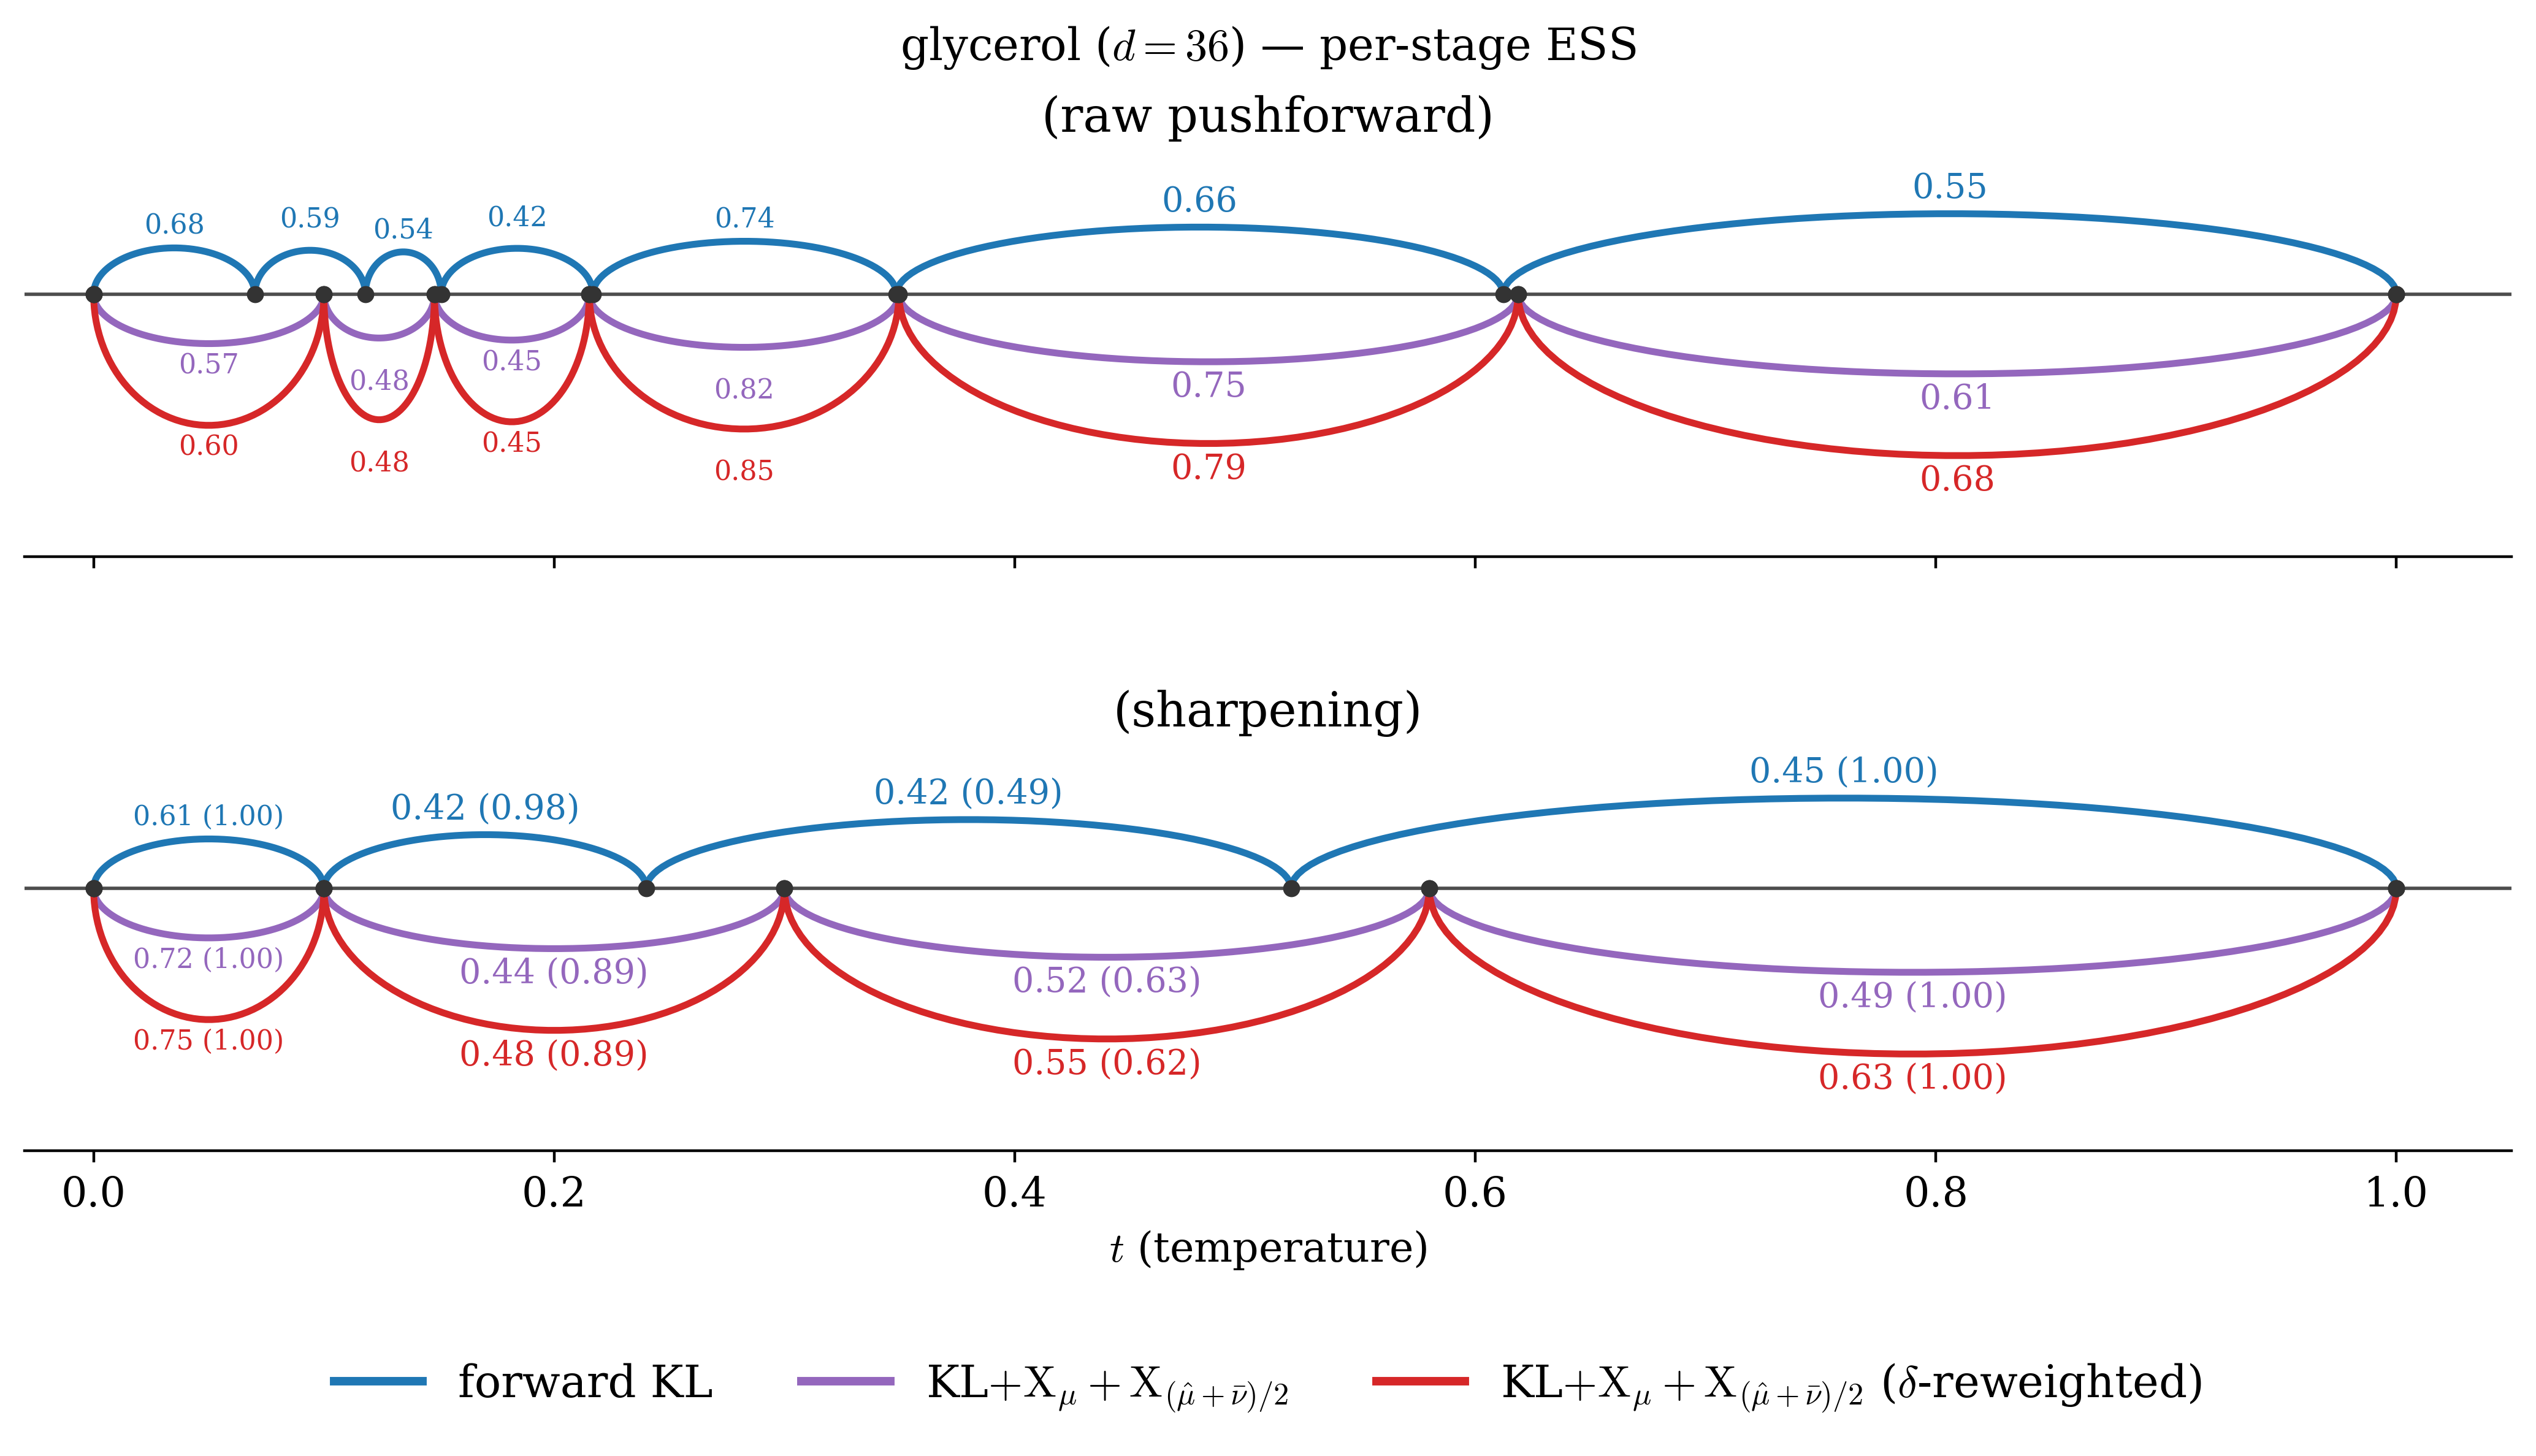
\includegraphics[width=\linewidth]{../glycerol_36d/ladder.png}
    \caption{Glycerol per-stage validation $\ESS$ as annealing-ladder arcs, raw (top) and sharpen (bottom).
    In each row forward KL is drawn above the axis (blue), $\KL{+}\X_\mu{+}\X_{(\hat\mu+\bar\nu)/2}$ below
    (purple), and its $\delta$-reweighted variant further below (red). Each arc is an accepted stage; the apex
    label is that stage's validation $\ESS$; a cross marks a bridge the ladder failed to reach.}
    \label{fig: glycerol-ladder}
\end{figure}

Glycerol is achiral (each torsion marginal is even, $p(\phi) = p(-\phi)$), and every rotatable torsion is
three-fold: gauche$^{\pm}$ near $\pm 60^\circ$ and trans near $180^\circ$. The $\pm\phi$ symmetry pairs
gauche$^{-}\!\leftrightarrow$\,gauche$^{+}$ and leaves trans self-symmetric, so the joint target over the five
rotatable torsions is combinatorially multimodal (dozens of conformers), which is what the wide-coverage pool
must cover.

\begin{figure}[htbp]
    \centering
    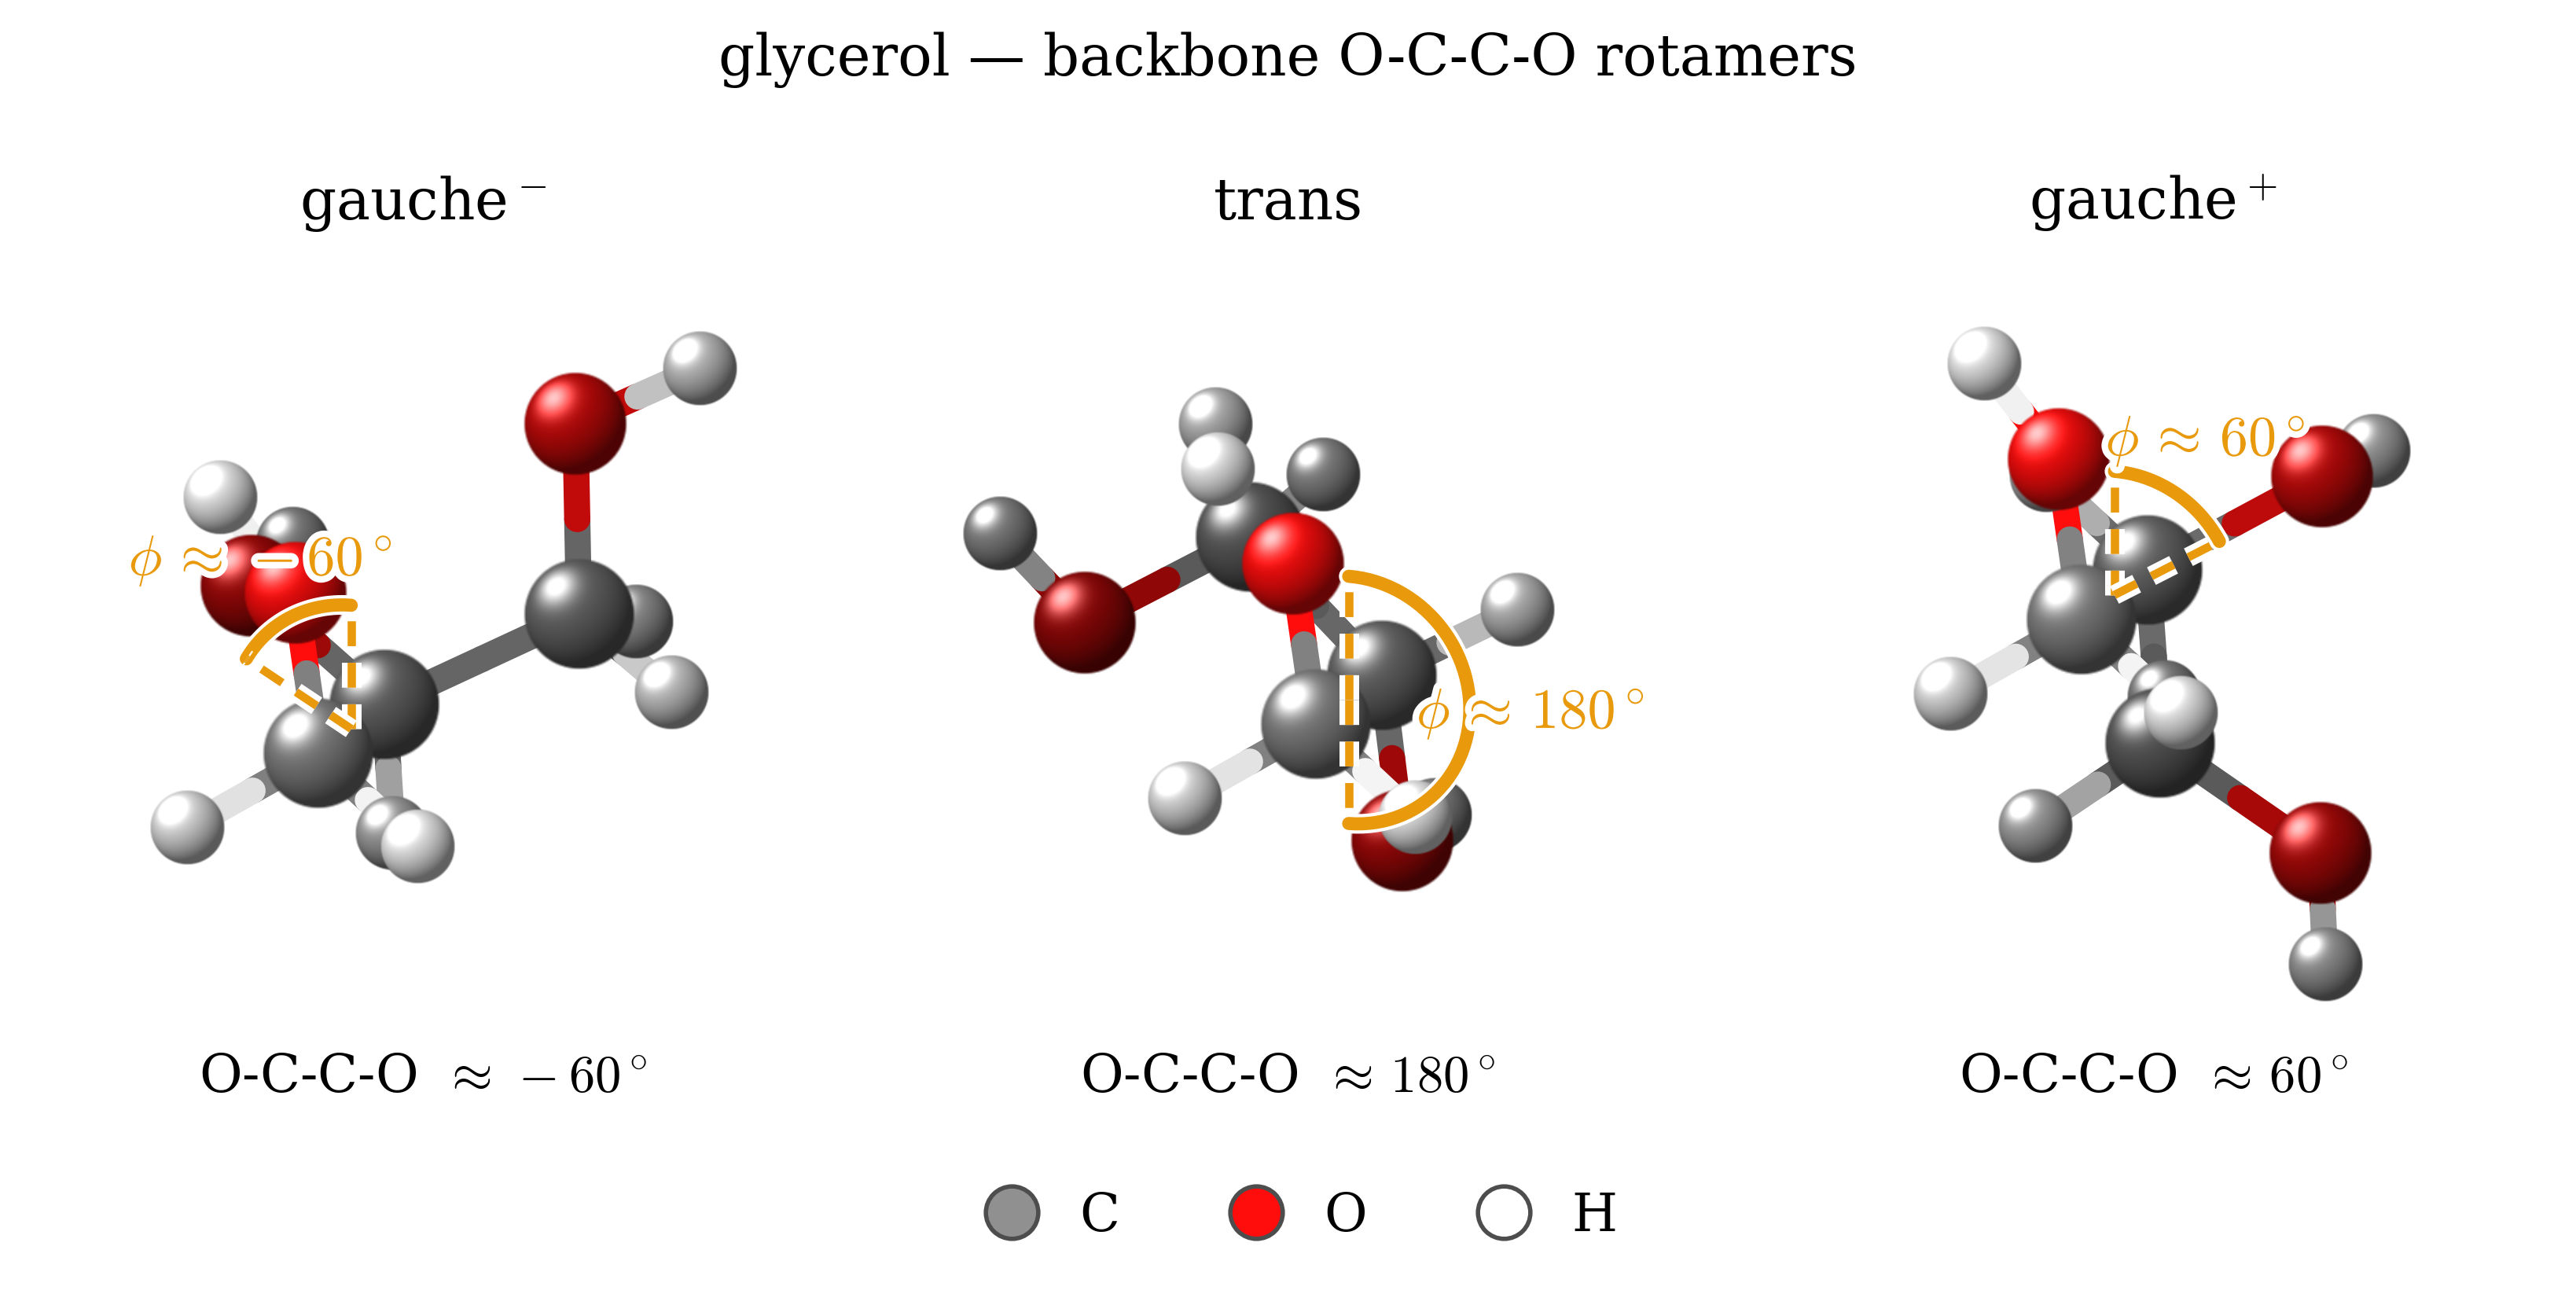
\includegraphics[width=\linewidth]{../glycerol_36d/conformers.png}
    \caption{Typical glycerol configurations at the three states of the backbone O--C--C--O torsion:
    gauche$^-$ ($-60^\circ$), trans ($180^\circ$), gauche$^+$ ($+60^\circ$). The gold arc marks the dihedral
    $\phi$; ball-and-stick (C grey, O red, H white). These are the rotamer wells that, taken in combination
    across the five rotatable torsions, make the target combinatorially multimodal.}
    \label{fig: glycerol-conformers}
\end{figure}

\begin{figure}[htbp]
    \centering
    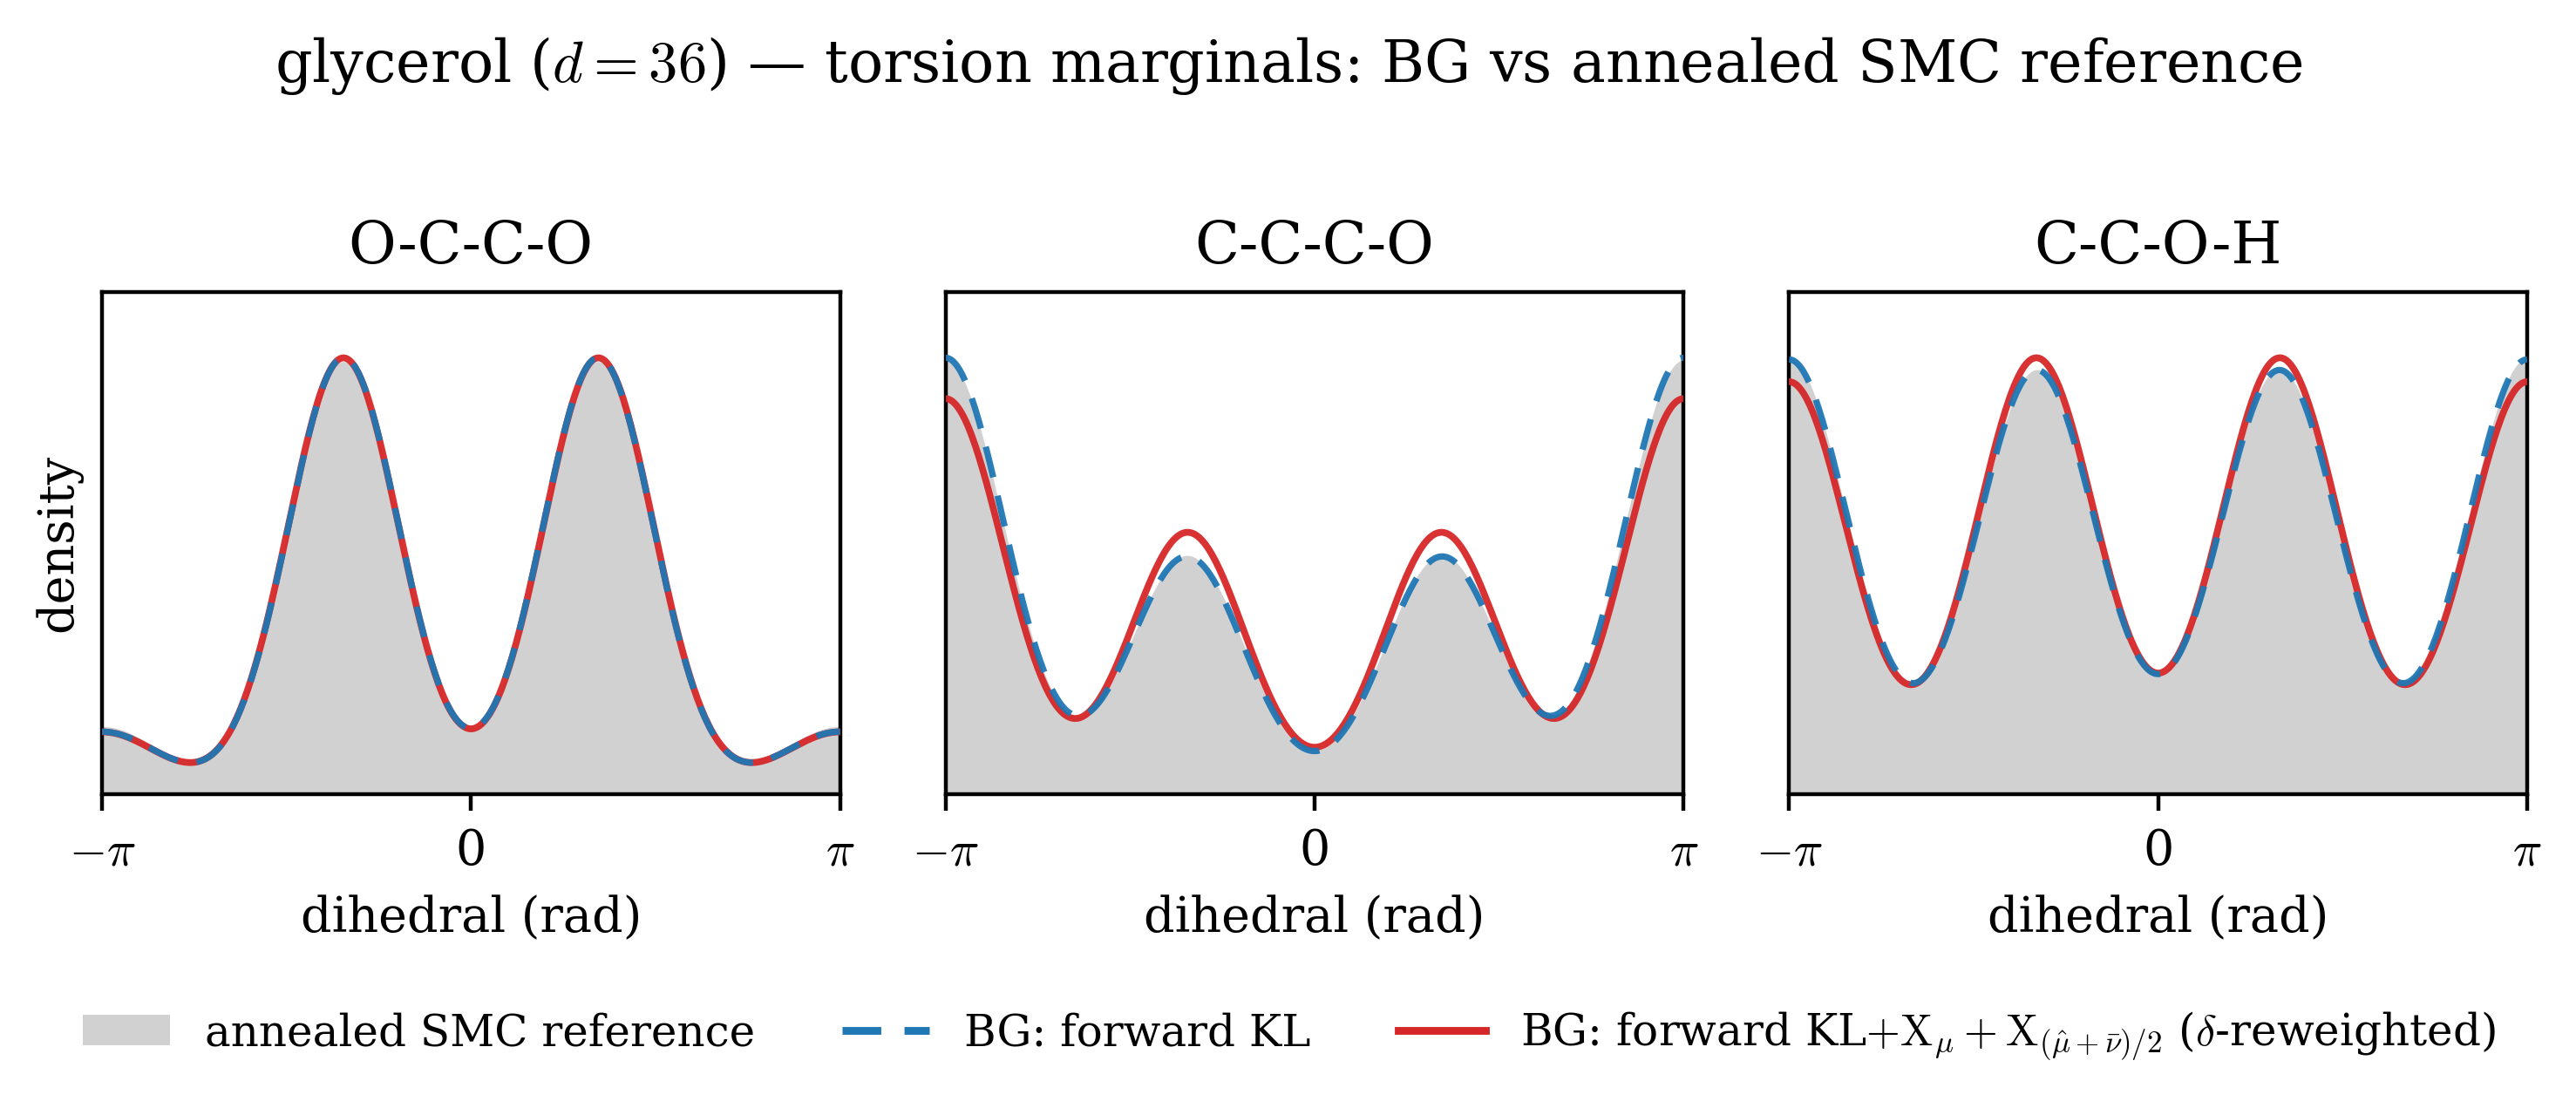
\includegraphics[width=\linewidth]{../glycerol_36d/dihedrals.png}
    \caption{Glycerol torsion marginals of both generators against a long, converged molecular-dynamics
    reference (grey; a batched Langevin on the same target, $2\times10^5$ walkers run to convergence): forward
    KL (blue) and $\KL{+}\X_\mu{+}\X_{(\hat\mu+\bar\nu)/2}$, $\delta$-reweighted (red) --- both sharpened, the
    cap annealed to $e = 200$. Because the torsion marginals are insensitive to the soft cap (steric clashes
    are unpopulated at equilibrium), this reference coincides with the bare-Amber torsion distribution. Both
    generators recover the multimodal gauche$^{\pm}$/trans structure of the
    characteristic glycerol torsions, evidence that they sample the target rather than collapsing onto a single
    well.}
    \label{fig: glycerol-dihedrals}
\end{figure}

\FloatBarrier
\subsubsection{Diethanolamine ($d = 48$)}
\label{sec: dea}

We test the generator on the full internal-coordinate diethanolamine target (\mbox{HN(CH$_2$CH$_2$OH)$_2$},
$d = 48$), comparing the two best losses under the same sharpening schedule (the soft cap geometrically
annealed $e\!:\!100\!\to\!200$, a Monte-Carlo sharpening step per stage): forward KL, and the $\X$-regularized
$\KL{+}\X_\mu{+}\X_{(\hat\mu+\bar\nu)/2}$ with the $\delta$-reweighted quench and temper ($\delta = 0.1$).
Forward KL reaches $t = 1$ in $K = 6$ stages, the $\X$-regularized loss in $K = 5$ (a single direct
$0.65 \to 1$ step), both on a single RTX~5070~Ti.

\begin{table}[h]
    \centering
    \small
    \begin{tabular}{@{}lccc@{}}
        \toprule
        loss & $K$ & wall (min) & $F$ \\
        \midrule
        annealed SMC                                            & 10 & 7 & 1455.44 \\
        forward KL                                              & 6 & 896 & 92.60 \\
        $\KL{+}\X_\mu{+}\X_{(\hat\mu+\bar\nu)/2}$, $\delta$-rw. & 5 & 782 & \textbf{35.90} \\
        \bottomrule
    \end{tabular}
    \caption{Diethanolamine ($d = 48$): two trained-flow losses and a no-flow annealed-SMC reference, all with
    a per-stage Monte-Carlo sharpening reweight (cap $e$ geometrically annealed $100 \to 200$): ladder length
    $K$, training wall-clock, and the error-propagation factor $F$ \eqref{eq: F} (smaller better; $F$ includes
    the sharpening reweight). All wall-clock times are on a single RTX~5070~Ti. $\delta$-rw.\ $=$
    $\delta$-reweighted quench and temper.}
    \label{tab: dea}
\end{table}

The $\X$-regularized loss with $\delta$-reweighting reaches $F = 35.9$ versus forward KL's $F = 92.6$ --- a
$\sim$$2.6\times$ reduction in importance-weight waste at identical settings (glycerol showed a comparable
$\sim$$3.1\times$ gap, $14.2$ vs $44.0$). The advantage shows in the late, sharp stages and in the ladder
length: forward KL's per-stage validation $\ESS$ stalls at $0.46$--$0.53$ and it needs $6$ rungs to reach
$t = 1$, whereas the $\X{+}\delta$ run holds a higher $\ESS$ ($0.74$ on the final, direct $0.65 \to 1$ step) and
reaches $t = 1$ in $5$ (Fig.~\ref{fig: dea-ladder}). This is a singular, high-dimensional, combinatorially
multimodal target, so each run is a multi-hour computation; that the $\X$-regularized loss closes it on a
single consumer GPU --- not a datacenter accelerator --- is the practical point.

\begin{figure}[htbp]
    \centering
    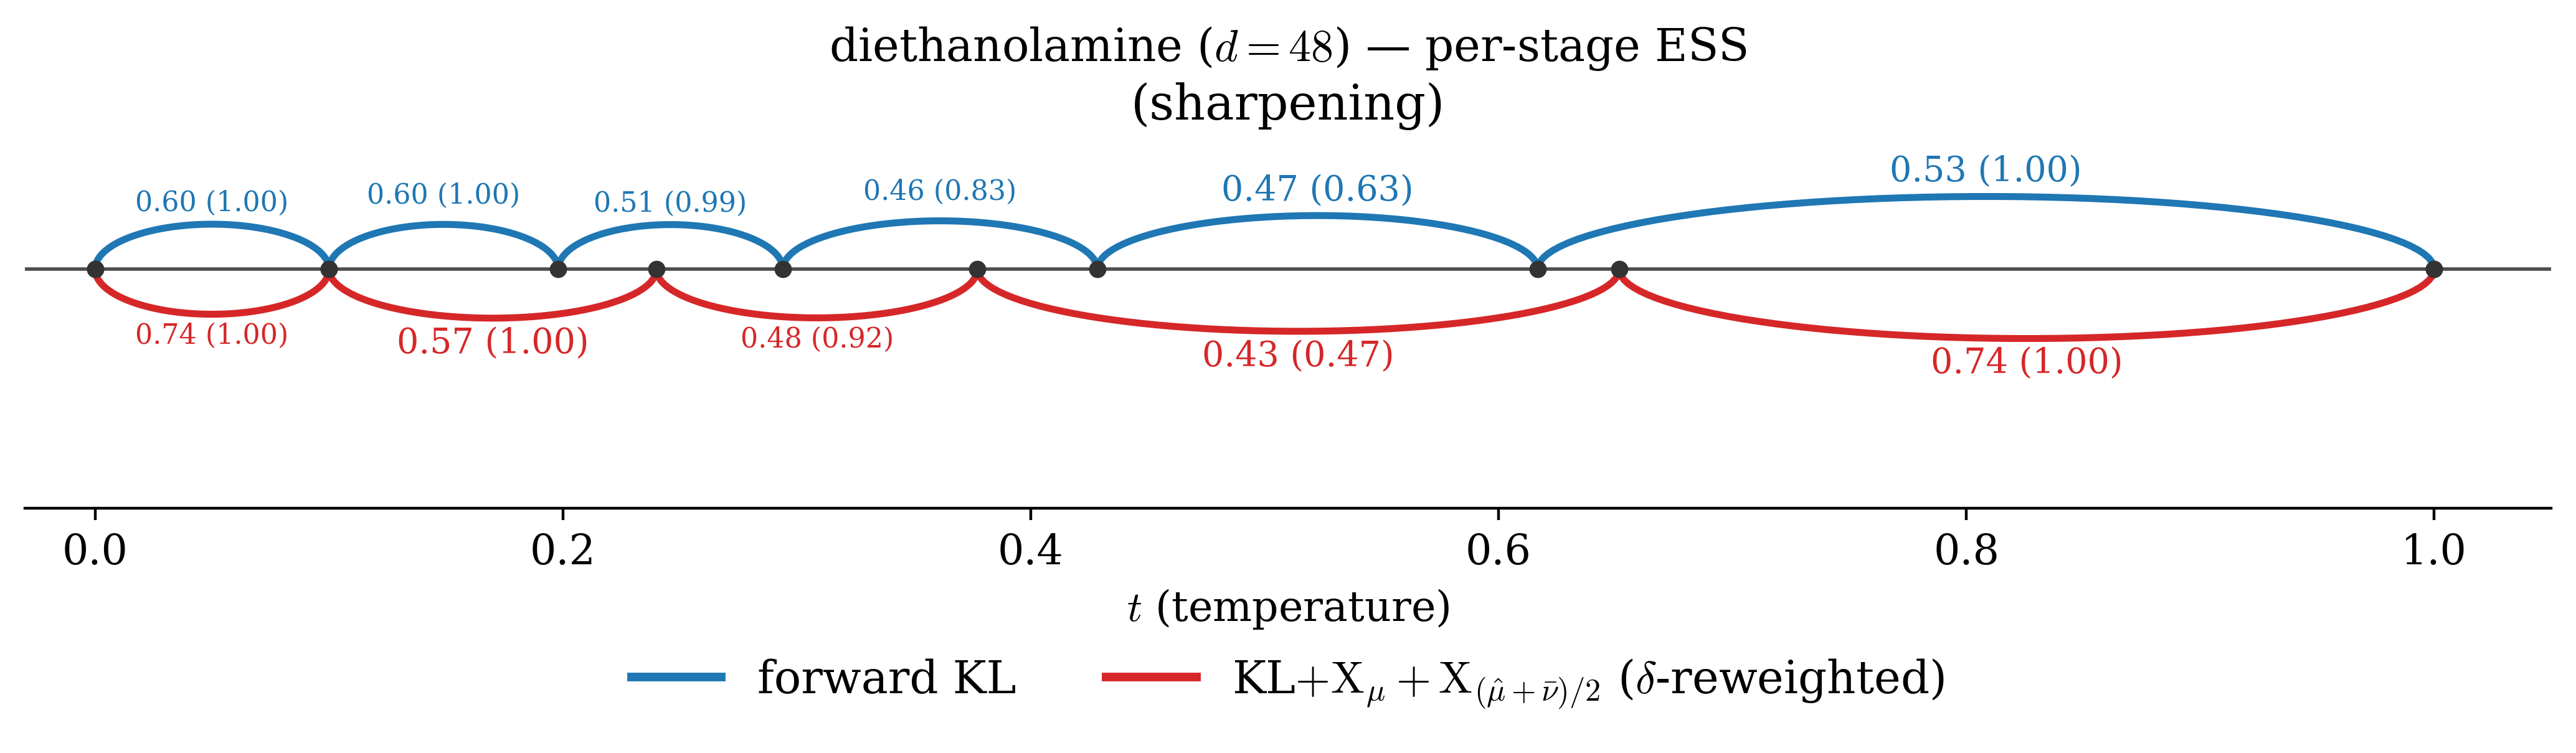
\includegraphics[width=\linewidth]{../diethanolamine_48d/ladder.png}
    \caption{Diethanolamine per-stage $\ESS$ as annealing-ladder arcs (sharpening schedule): forward KL above
    the axis (blue), $\KL{+}\X_\mu{+}\X_{(\hat\mu+\bar\nu)/2}$, $\delta$-reweighted, below (red). Each arc is an
    accepted stage; the apex label is that stage's validation $\ESS$, with the sharpening $\ESS$ in
    parentheses.}
    \label{fig: dea-ladder}
\end{figure}

Diethanolamine has a plane of symmetry (each torsion marginal is even, $p(\phi) = p(-\phi)$); its rotatable
backbone torsions --- O--C--C--N and C--C--N--C along the ethanolamine arms, plus the hydroxyl rotations ---
are each multi-well (gauche$^{\pm}$/trans), so the joint target is combinatorially multimodal, which the
wide-coverage pool must cover.

\begin{figure}[htbp]
    \centering
    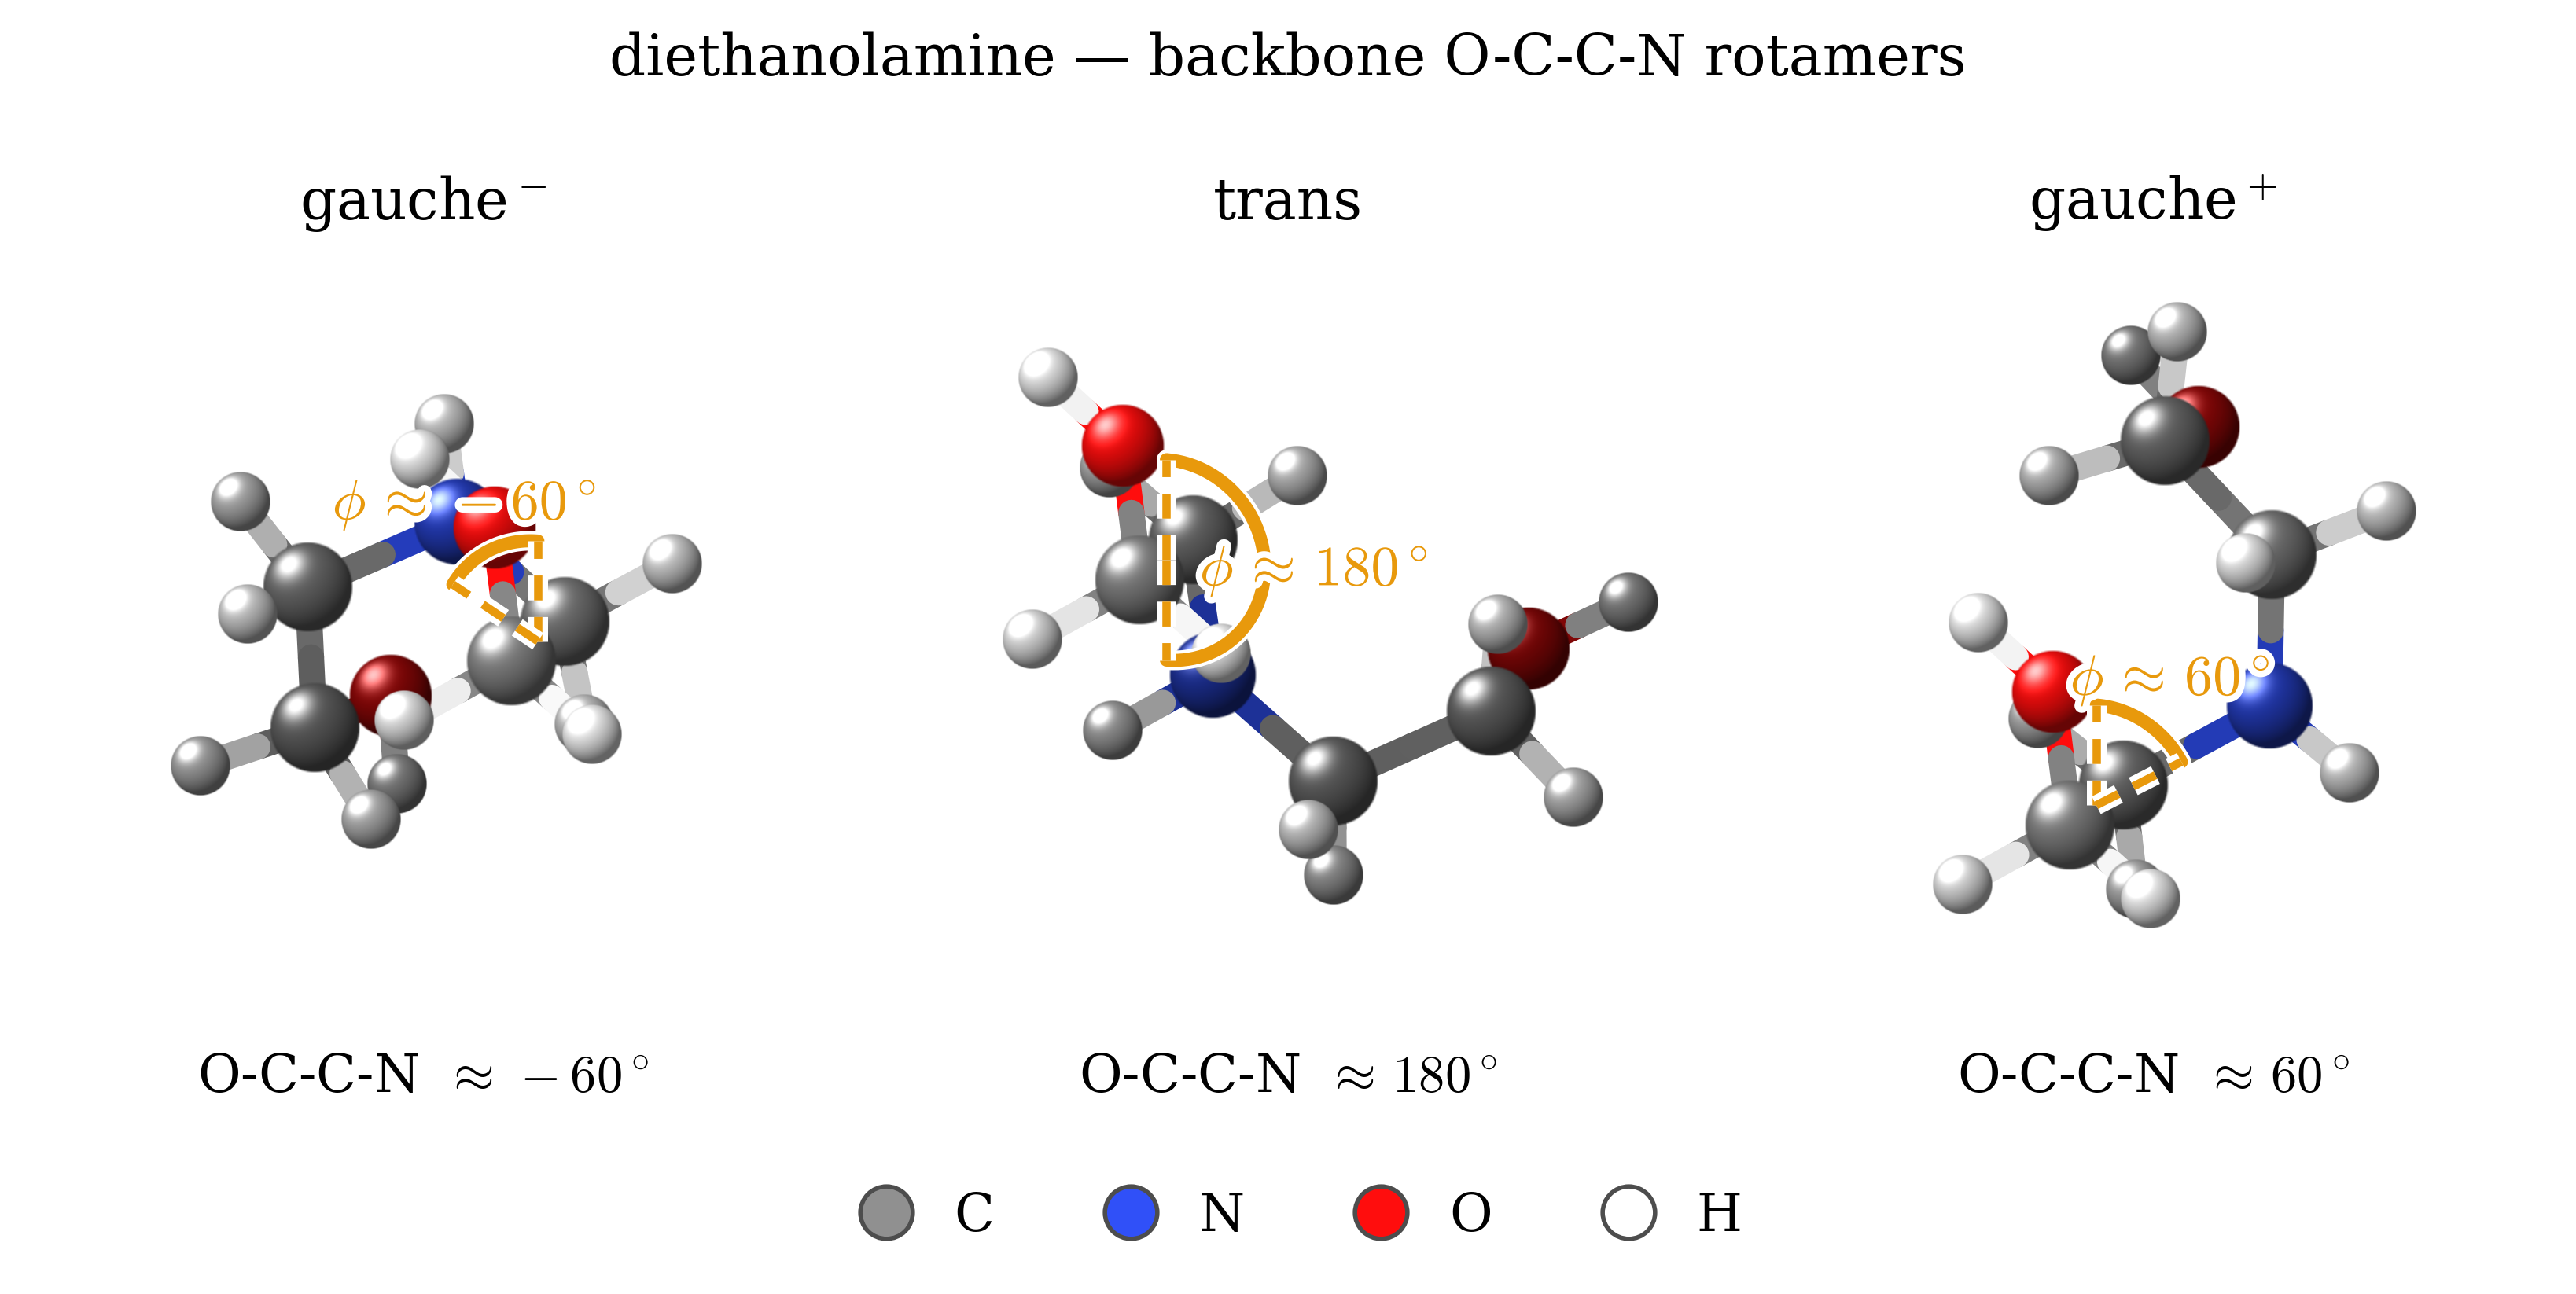
\includegraphics[width=\linewidth]{../diethanolamine_48d/conformers.png}
    \caption{Typical diethanolamine configurations at the three states of a backbone O--C--C--N torsion:
    gauche$^-$ ($-60^\circ$), trans ($180^\circ$), gauche$^+$ ($+60^\circ$). The gold arc marks the dihedral
    $\phi$; ball-and-stick (C grey, N blue, O red, H white).}
    \label{fig: dea-conformers}
\end{figure}

\begin{figure}[htbp]
    \centering
    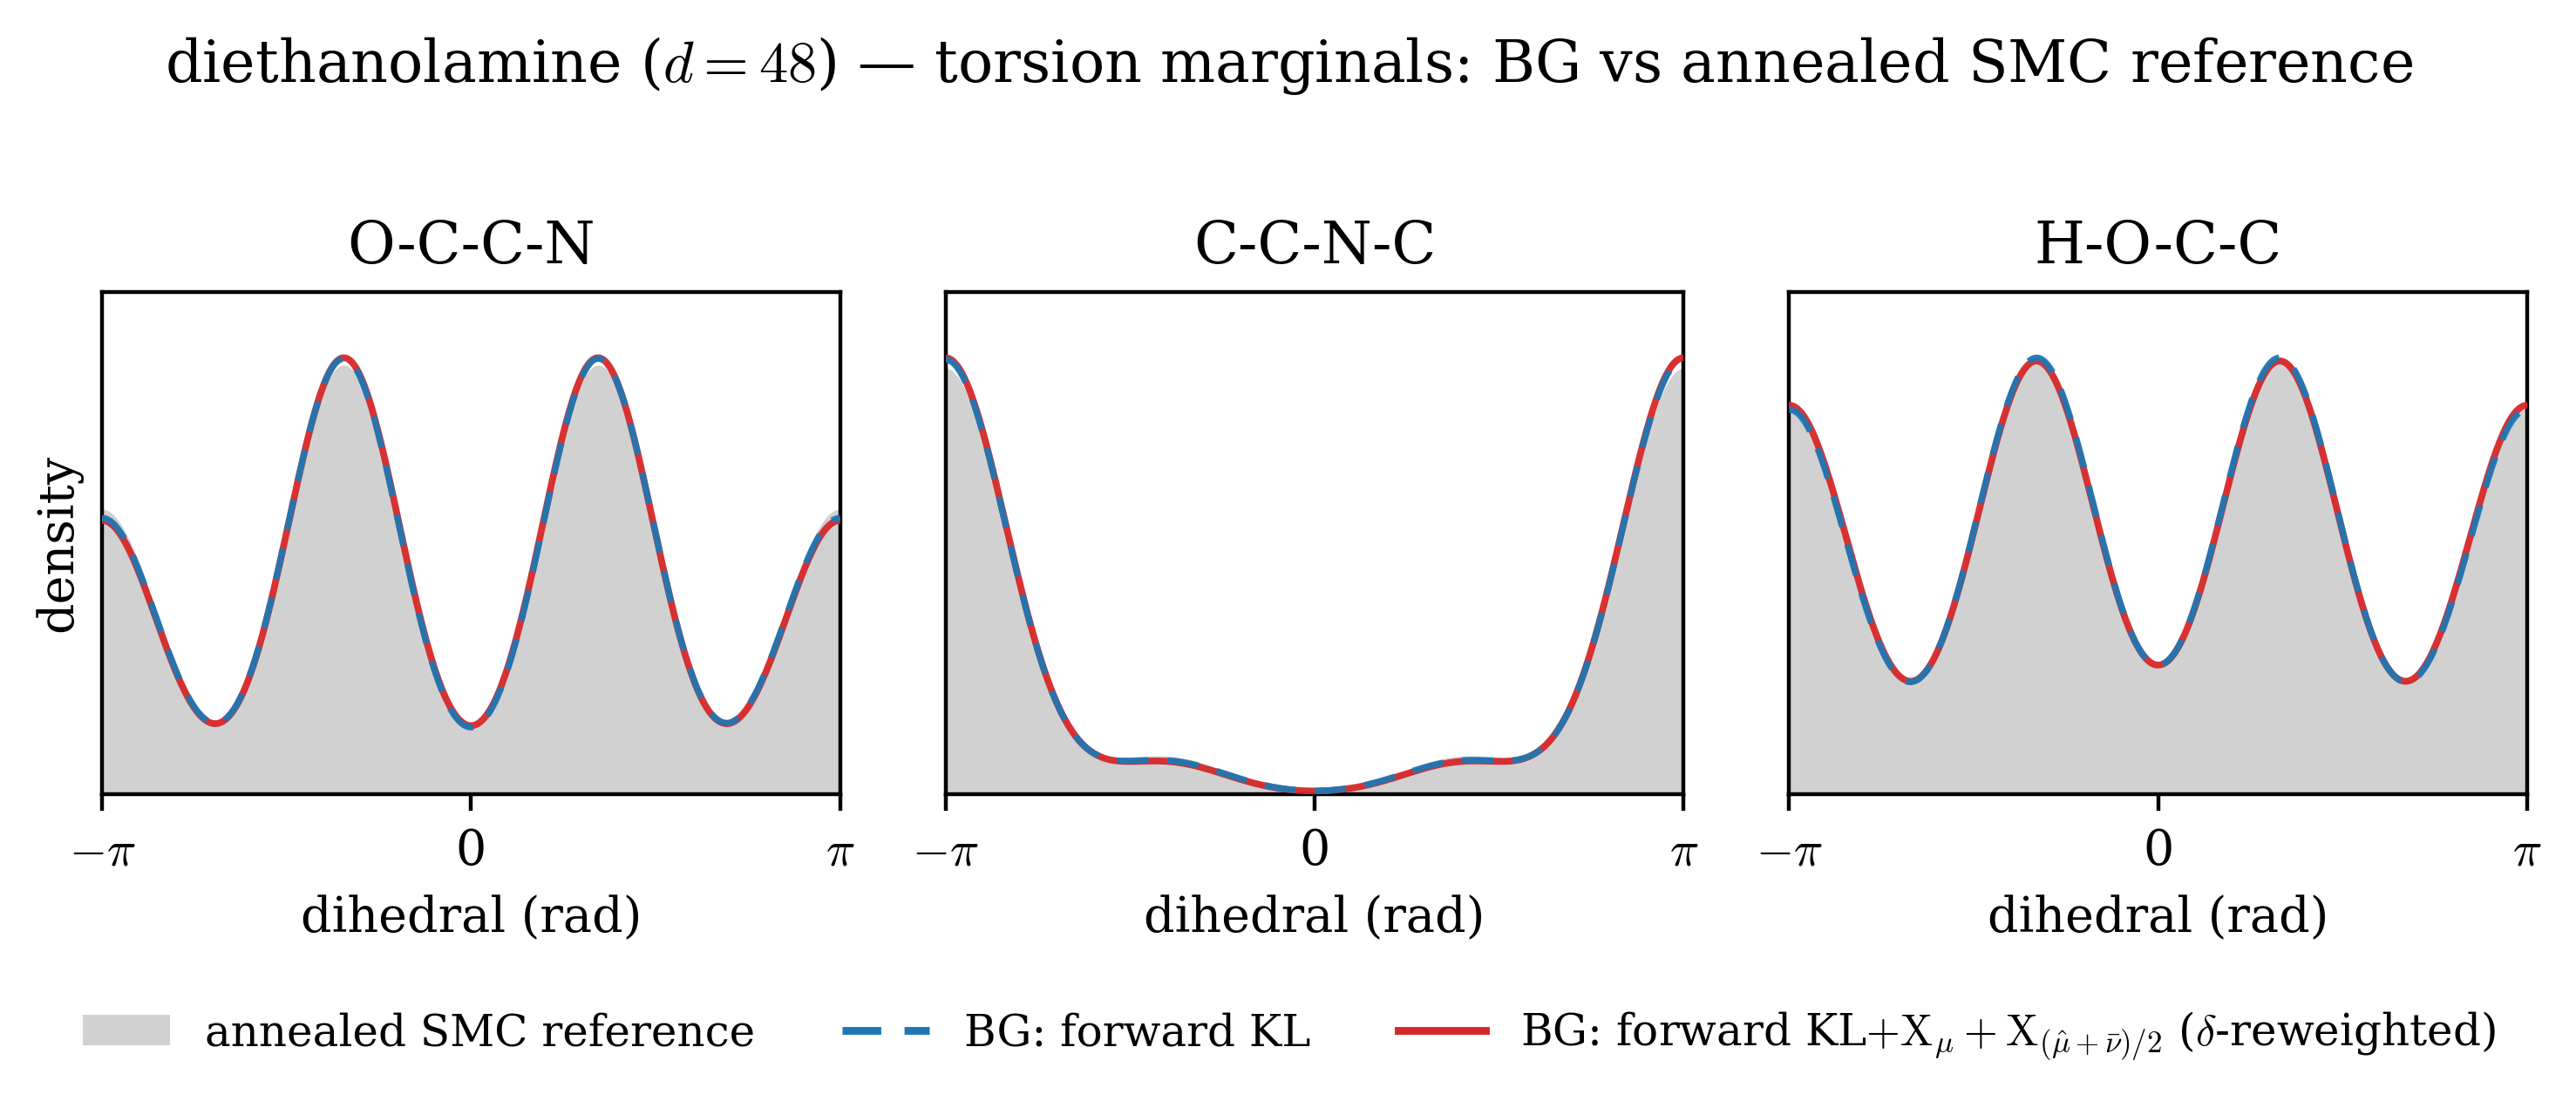
\includegraphics[width=\linewidth]{../diethanolamine_48d/dihedrals.png}
    \caption{Diethanolamine torsion marginals of both generators against a long, converged molecular-dynamics
    reference (grey; a batched Langevin on the same target, $2\times10^5$ walkers): forward KL (blue) and
    $\KL{+}\X_\mu{+}\X_{(\hat\mu+\bar\nu)/2}$, $\delta$-reweighted (red) --- both sharpened, the cap annealed to
    $e = 200$. Both recover the multimodal backbone torsions and track the MD reference, evidence that they
    sample the target rather than collapsing onto a single well.}
    \label{fig: dea-dihedrals}
\end{figure}

Against the MD reference (Fig.~\ref{fig: dea-dihedrals}) the two losses are visually indistinguishable --- both
recover the multimodal backbone torsions and neither is discernibly closer to MD. The separation is in
efficiency, not in the sampled marginals: $\KL{+}\X$ reaches $t = 1$ in fewer stages ($5$ vs $6$) with a higher
final-step $\ESS$ ($0.74$ vs $0.53$), a $\sim 2.6\times$ smaller error-propagation factor ($F = 35.9$ vs
$92.6$), and fewer rejected stage attempts in the early ladder (stages 2--4: $1,1,0$ rejections versus forward
KL's $2,2,1$). Switching the trained flow off entirely --- the identity map at every stage, i.e.\ plain
adaptive annealed SMC over the same ladder --- gives $F = 1455$ in $K = 10$ stages. The trained
$\X$-regularized flow therefore cuts the propagation factor by $\sim$$40\times$ and halves the ladder length
($5$ vs $10$): on this singular target the transport map adds even more over annealing alone than on glycerol,
the practical justification for training a flow at all.

\FloatBarrier
\subsubsection{Alanine dipeptide ($d = 60$)}
\label{sec: adp}

We push the generator to alanine dipeptide (ADP, Ac--Ala--NHMe), the canonical Boltzmann-generator benchmark,
in full internal coordinates ($d = 60$). The qualitative step up from glycerol and diethanolamine is the
target's character: those are dominated by smooth rotatable-bond multimodality, whereas ADP folds the backbone
tightly enough that the Lennard-Jones clash core --- not the torsion profile --- sets the hardest part of the
anneal. We report the $\X$-regularized loss only ($\KL{+}\X_\mu{+}\X_{(\hat\mu+\bar\nu)/2}$,
$\delta$-reweighted, $\delta = 0.1$), with a per-stage Monte-Carlo sharpening in which \emph{both} the cap
$e\!:\!100\!\to\!200$ and the clash floor $r_{\mathrm{floor}}\!:\!0.2\!\to\!0.1$ are annealed arithmetically
(the only target that anneals $r_{\mathrm{floor}}$). The run reaches $t = 1$ in $K = 11$ stages at $F = 67.9$,
with every stage holding validation $\ESS \ge 0.51$ and sharpening $\ESS \ge 0.95$
(Table~\ref{tab: adp}, Fig.~\ref{fig: adp-ess}).

\begin{table}[h]
    \centering
    \small
    \begin{tabular}{@{}lccc@{}}
        \toprule
        loss & $K$ & wall (min) & $F$ \\
        \midrule
        annealed SMC                                           & 12 & 23  & 129.70 \\
        $\KL{+}\X_\mu{+}\X_{(\hat\mu+\bar\nu)/2}$, $\delta$-rw. & 11 & ${\sim}1000$ & \textbf{67.95} \\
        \bottomrule
    \end{tabular}
    \caption{Alanine dipeptide ($d = 60$), the $\X$-regularized loss with a per-stage Monte-Carlo sharpening
    reweight (the cap $e$ and floor $r_{\mathrm{floor}}$ annealed arithmetically): ladder length $K$,
    wall-clock, and the error-propagation factor $F$ \eqref{eq: F} (smaller better; $F$ includes the sharpening
    reweight). The first row is a no-flow annealed-SMC reference (identity map over the same ladder); the
    trained flow only halves $F$ here ($130 \to 68$), far less than the $20$--$40\times$ reduction on the
    lighter $d \le 48$ targets --- it earns little near ADP's clash singularity. The bare composed flow's
    end-to-end $\ESS$ against the sharp target is ${\sim}5\times10^{-6}$, so the per-stage SMC sharpening is the
    deliverable, not a raw pushforward. $\delta$-rw.\ $=$ $\delta$-reweighted quench and temper.}
    \label{tab: adp}
\end{table}

For comparison, the lighter targets close at $F = 14.2$ (glycerol) and $F = 35.9$ (diethanolamine) with the
same loss; ADP's larger $F$ is the price of its singular nonbonded core, not of its multimodality. Three
ADP-only factors nonetheless make this $F$ read smaller than a strict like-for-like extension of that trend:
the per-stage $\ESS$ is the smooth estimator of \S\ref{sec: mol-engineering} rather than the raw weighted
$\ESS$ (WSS); $r_{\mathrm{floor}}$ is annealed alongside the cap; and the ladder is much longer ($K = 11$
versus $4$ and $5$), its smaller per-step jumps keeping each per-stage $\ESS$ high. All three raise the
per-stage $\ESS$ entering $F$, and none applied to the lighter targets.

\begin{figure}[htbp]
    \centering
    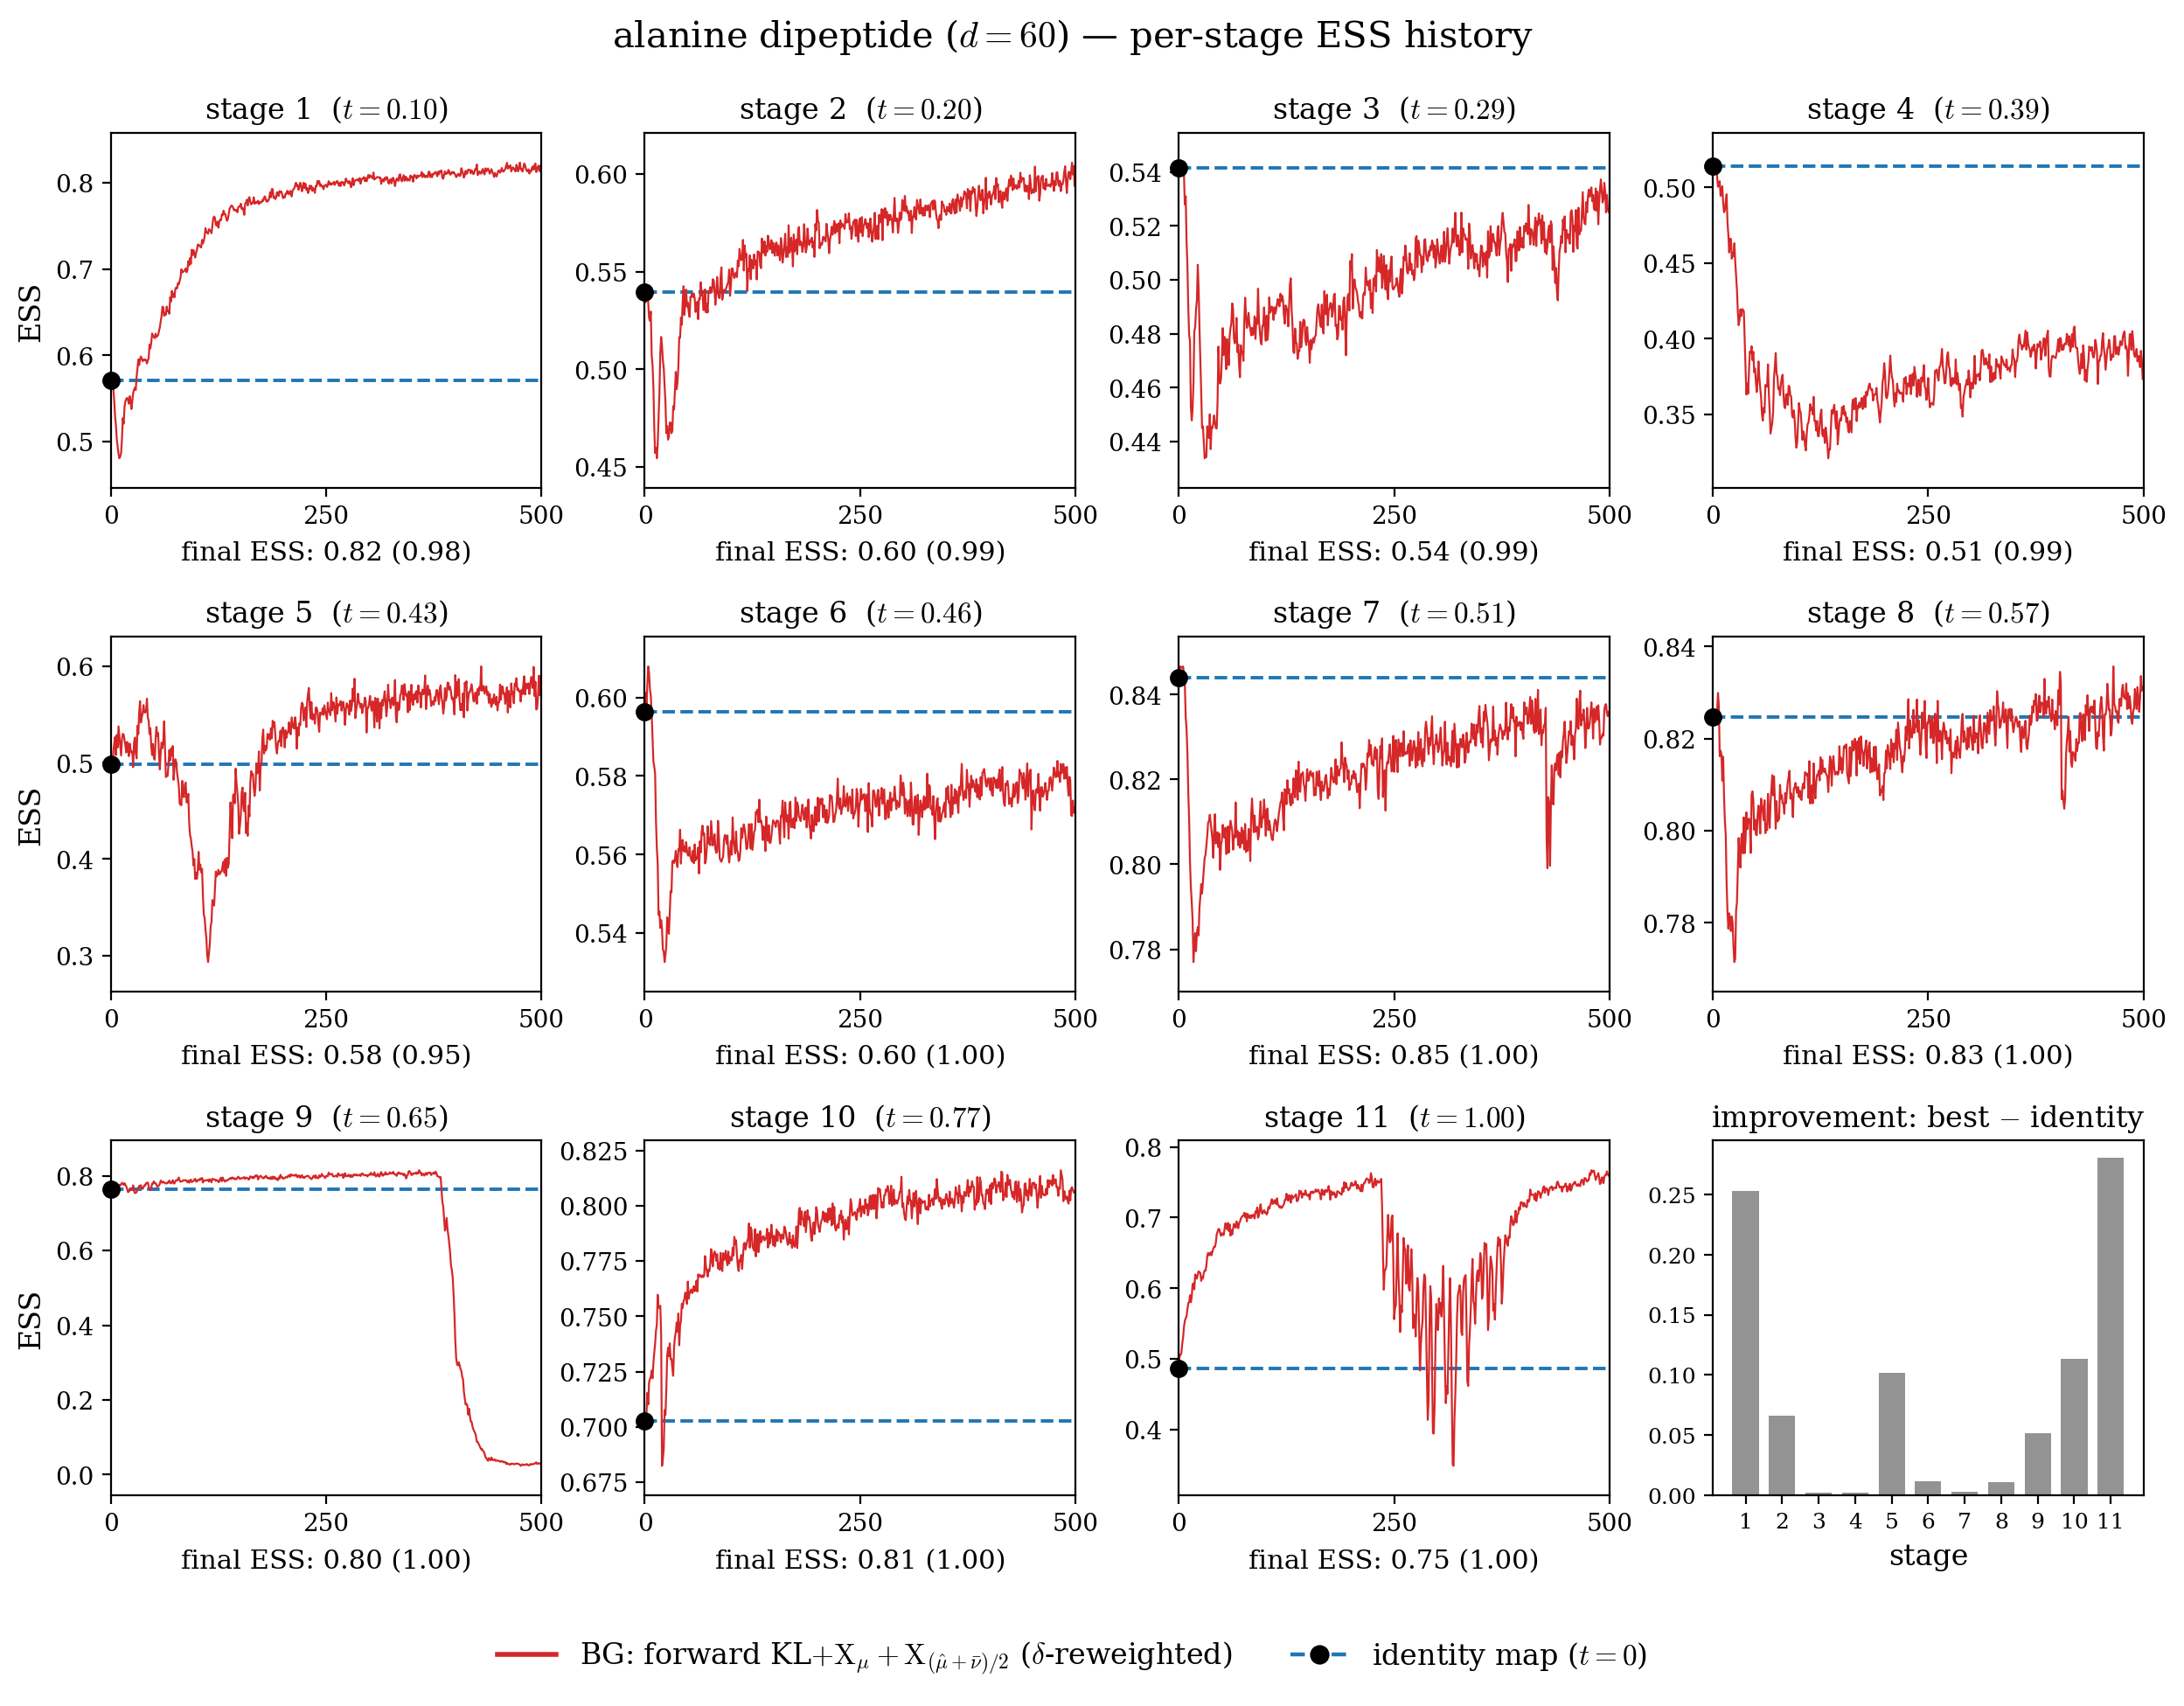
\includegraphics[width=\linewidth]{../adp_60d/ess_history.png}
    \caption{Alanine dipeptide per-stage $\ESS$ history: each panel is the per-step effective sample size
    during that stage's $\X$-regularized $\delta$-reweighted flow training (red), against the identity-map
    baseline at $t = 0$ (blue dashed). Below each panel is that stage's accepted validation $\ESS$ with the
    sharpening $\ESS$ in parentheses. Note the dip across $t \approx 0.29$--$0.46$ --- the clash bottleneck ---
    and the recovery to $\ESS \approx 0.8$ once the cap is sharp enough to separate the basins.}
    \label{fig: adp-ess}
\end{figure}

\paragraph{The $t \approx 0.3$--$0.45$ bottleneck.} The instability is sharply localized. The stages spanning
$t \approx 0.29$--$0.43$ (soft cap $e \approx 129$--$143$) are where the nonbonded core first bites: the run
minimum validation $\ESS$ ($0.51$ at $t = 0.39$) sits here, and these are the \emph{only} stages that shrink
the step ($n_{\mathrm{shrink}} = 1$ at stages $3,4,5$) or retry heavily (3 attempts at stages $5,6$). Below
$t \approx 0.3$ the torsions still dominate and the flow trains in a single attempt; above $t \approx 0.5$ the
cap is sharp enough that the basins separate cleanly and $\ESS$ recovers to ${\approx}0.8$. The binding
constraint for ADP is the clash singularity, not the multimodality --- the qualitative difference from the
$d \le 48$ molecules, and the reason the three devices of \S\ref{sec: mol-engineering} (particle drop,
best-$\ESS$ gate snapshots, $r$-floor anneal), inert on glycerol and diethanolamine, were necessary here.

\paragraph{A key observation (open difficulty).} The per-stage $\ESS$ history (Fig.~\ref{fig: adp-ess})
exposes two coupled instabilities that the best-$\ESS$ gate works around but does not cure. First, the
within-stage $\ESS$ is \emph{non-monotone and unstable}: it can rise, plateau, then drop abruptly --- the sharp
collapse late in the $t = 0.65$ stage and the volatility at $t = 1$ are the clearest cases --- so the last
training step is frequently far below the best (stage~9's training $\ESS$ decays to $0.03$ by step $500$ while
the best-$\ESS$ gate keeps a snapshot at validation $\ESS = 0.80$). Second, near the clash bottleneck ($t \approx 0.3$--$0.5$)
several flows \emph{degenerate toward the identity map}: the best achievable $\ESS$ barely exceeds the $t = 0$
no-flow baseline ($\Delta = \text{best} - \text{identity} \approx 0$ at stages $3, 4, 7$), i.e.\ training fails
to improve on doing nothing. Both are understood consequences of the \emph{singularity of the potential} ---
the Lennard-Jones $r \to 0$ divergence leaves the soft-capped target ill-conditioned exactly where the
nonbonded core first bites, so the gradient signal that would pull the flow off identity is weakest there. We
report this as a known limitation; robust remedies (stronger or adaptive regularization annealing,
parameterizations tailored to the repulsive wall) are left to future work.

\begin{figure}[htbp]
    \centering
    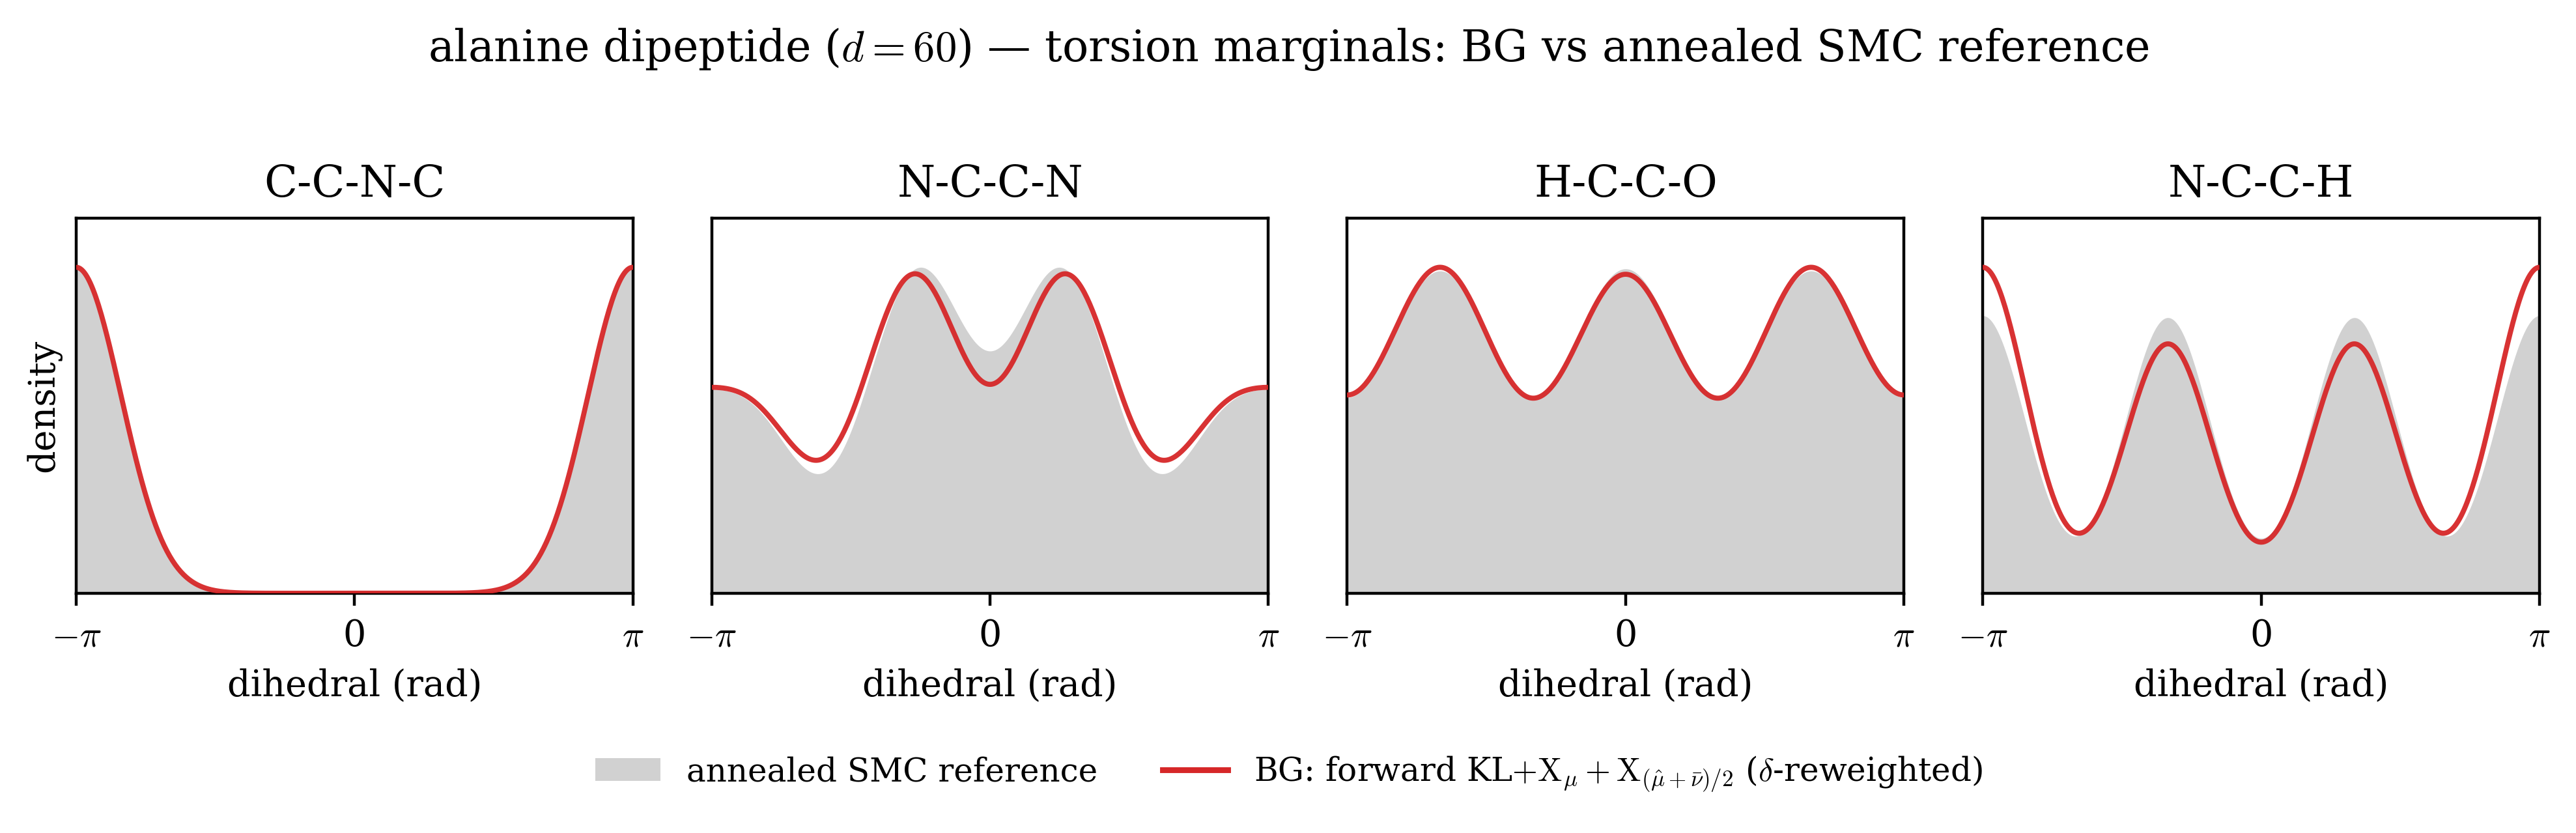
\includegraphics[width=\linewidth]{../adp_60d/dihedrals.png}
    \caption{Alanine dipeptide torsion marginals of the BG deliverable (red) against a long, converged
    molecular-dynamics reference (grey; batched Langevin on the same sharp target, $2\times10^5$ walkers). The
    four most multimodal proper torsions are shown; the densities are $\pm\phi$-symmetrised (the achiral target
    has $p(\phi) = p(-\phi)$). The BG recovers the multimodal backbone torsions and tracks MD; the peptide
    $\omega$ (C--C--N--C) is trans-dominant in the generator, the one torsion whose high rotation barrier also
    makes the uniform-init MD reference slow to converge.}
    \label{fig: adp-dihedrals}
\end{figure}

\paragraph{Multimodality and the L/D mirror.} ADP's backbone $\phi,\psi$ are multi-basin
(Fig.~\ref{fig: adp-dihedrals}). A second, ADP-specific feature is chirality: the classical force field is
mirror-symmetric (every term in \eqref{eq: amber} is invariant under reflection), so the L- and D-forms are
isoenergetic. A physical MD trajectory stays in one form --- inverting the $\mathrm{C}_\alpha$ needs bond
breaking --- but the internal-coordinate flow carries no chirality constraint and emits \emph{both}
(Fig.~\ref{fig: adp-conformers}). In the
Ramachandran (Fig.~\ref{fig: adp-rama}) this appears as the $(\phi,\psi)\!\to\!(-\phi,-\psi)$ point symmetry:
the D-basins are the exact mirror of the L-basins, each populated, where a single kinetically trapped physical
trajectory would show only one.

\begin{figure}[htbp]
    \centering
    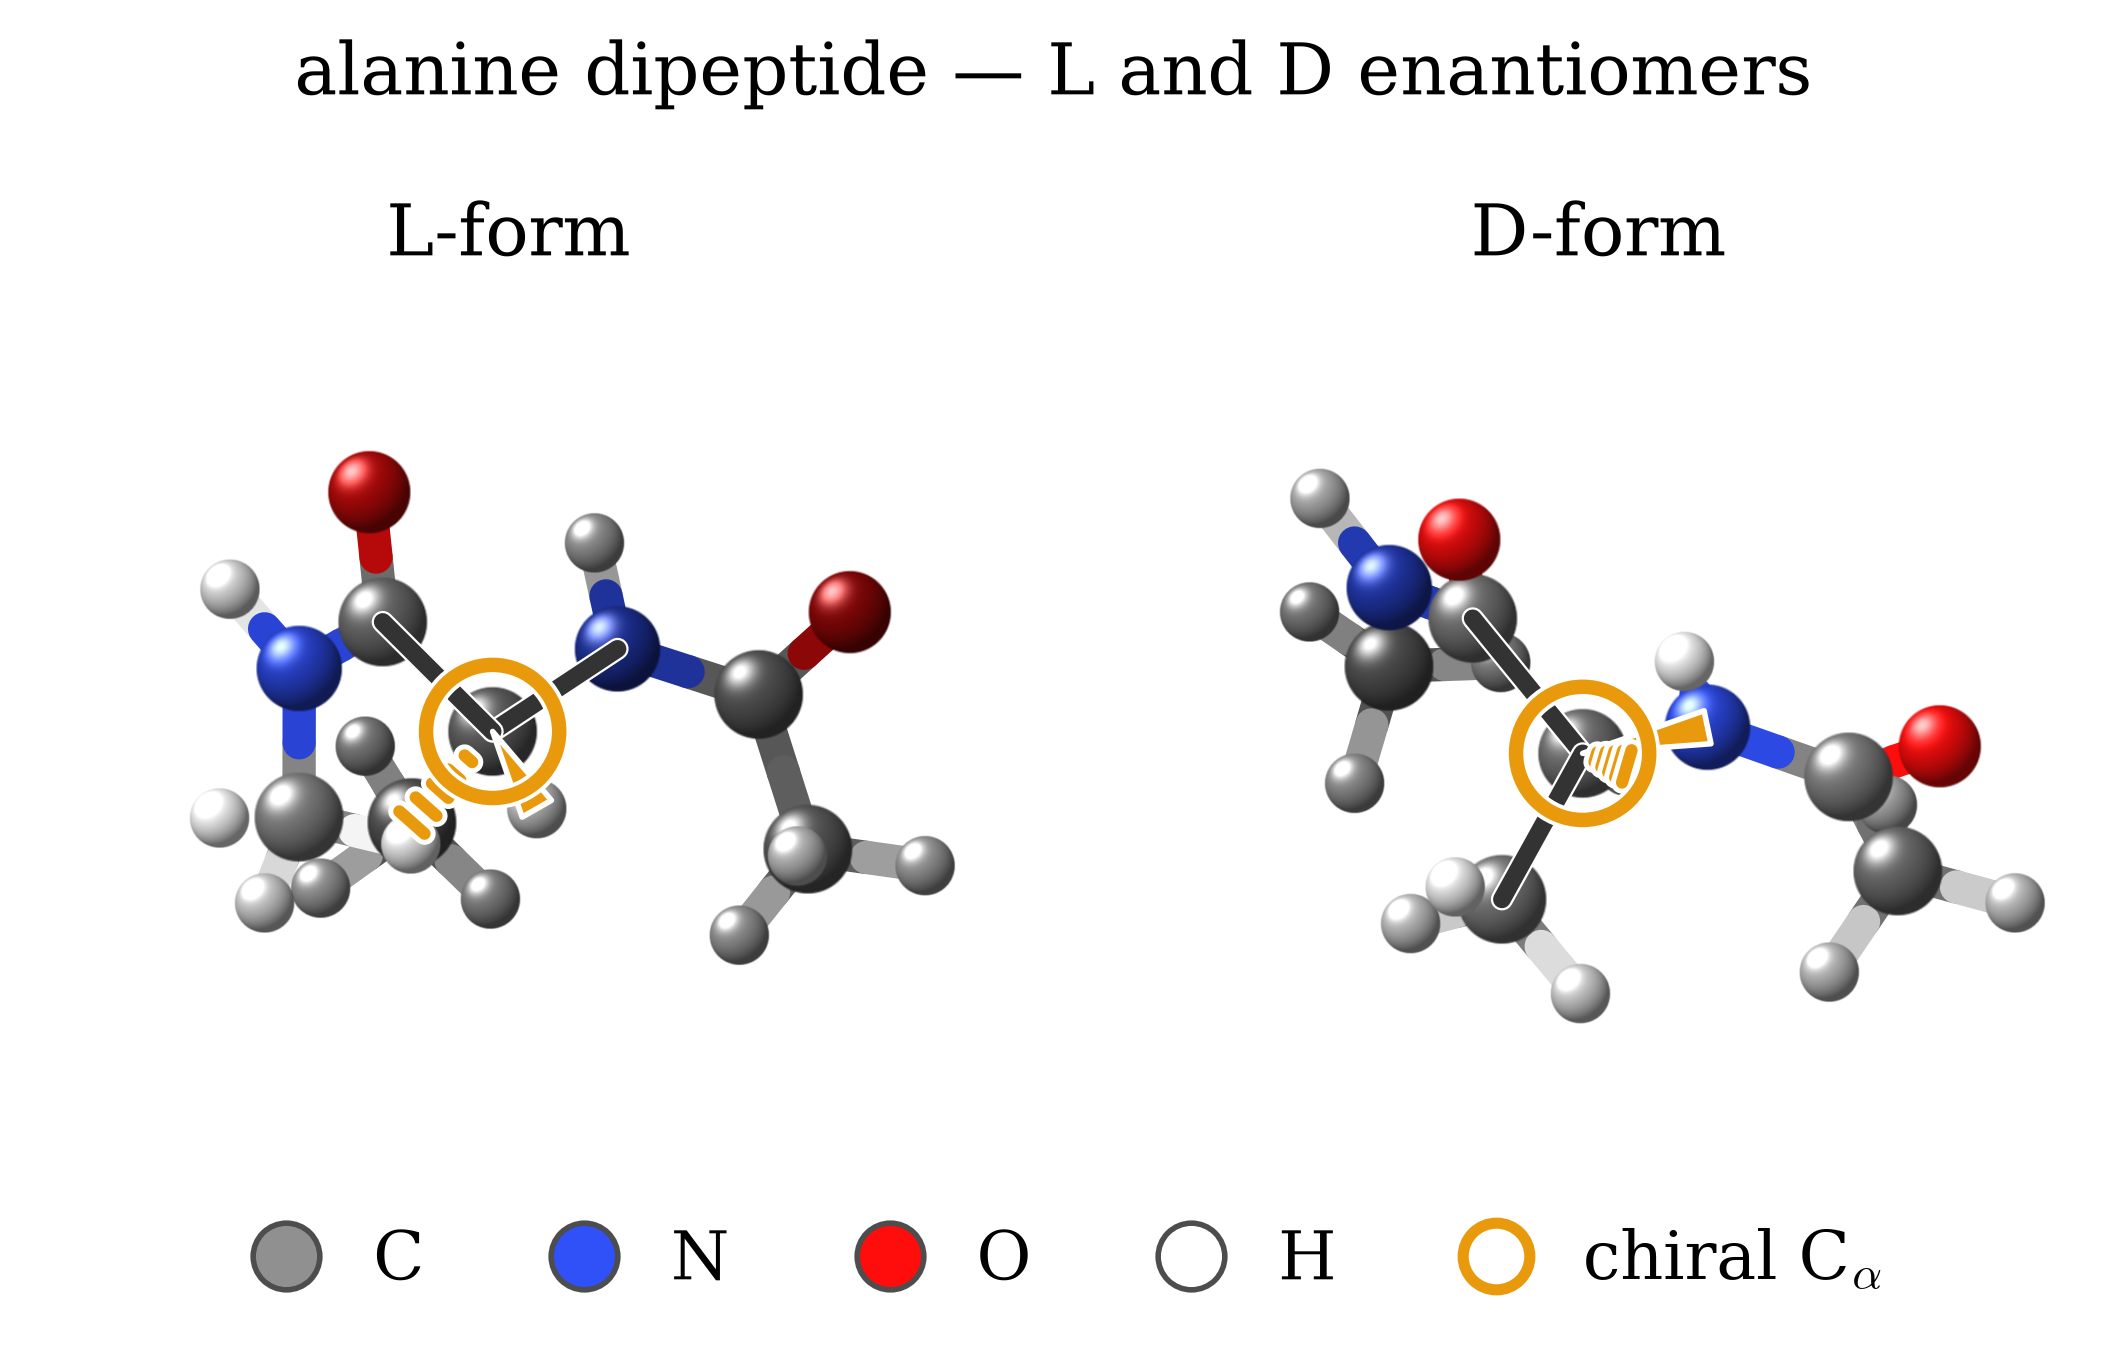
\includegraphics[width=0.74\linewidth]{../adp_60d/conformers.png}
    \caption{The two enantiomers of alanine dipeptide: the energy-minimized L-form and the D-form (a 3D
    reflection of it), shown from different viewpoints (ball-and-stick; C grey, N blue, O red, H white). The
    chiral $\mathrm{C}_\alpha$ is ringed in gold with stereo bonds (solid wedge toward the viewer, hashed
    behind), making the opposite handedness explicit in each panel. The achiral Amber force field makes the
    two isoenergetic, so the internal-coordinate generator emits both ---
    the structural companion to the $(\phi,\psi)\!\to\!(-\phi,-\psi)$ Ramachandran symmetry of
    Fig.~\ref{fig: adp-rama}.}
    \label{fig: adp-conformers}
\end{figure}

\begin{figure}[htbp]
    \centering
    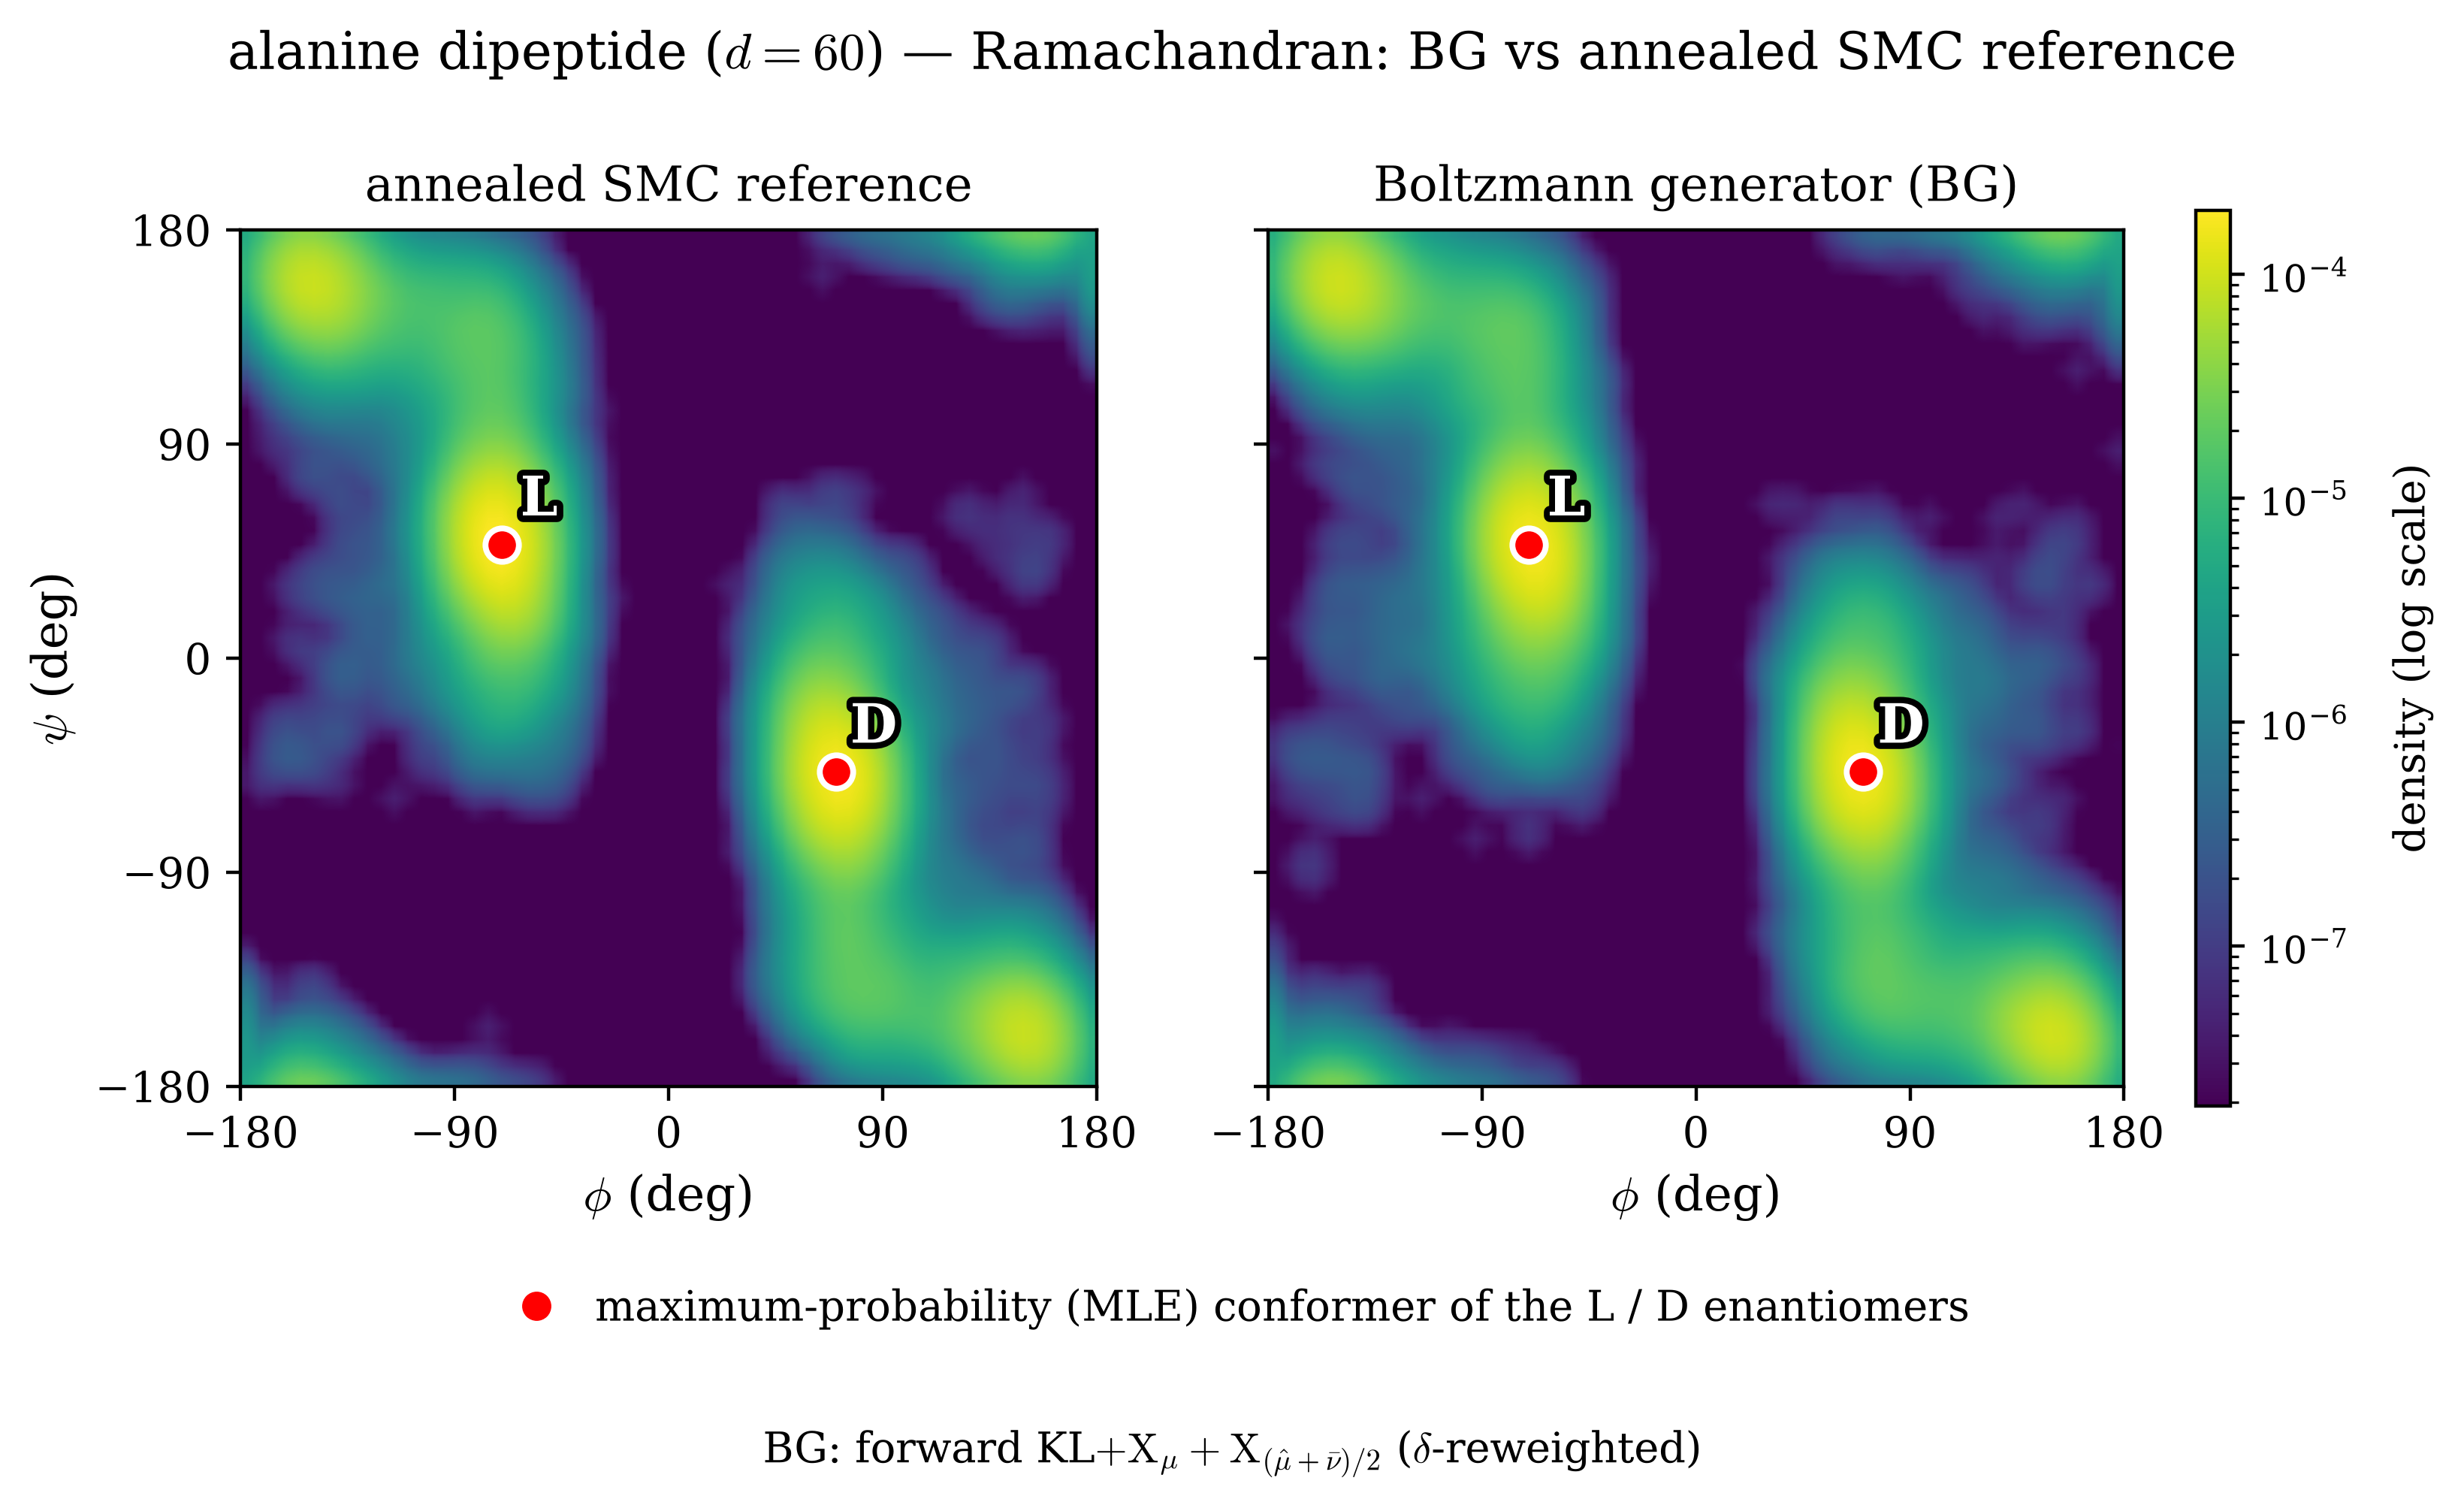
\includegraphics[width=0.92\linewidth]{../adp_60d/ramachandran.png}
    \caption{Alanine dipeptide Ramachandran ($\phi$--$\psi$), shared log-density scale: the BG deliverable
    (right) against the annealed-SMC reference (left). Red dots mark the maximum-probability (MLE) conformer of
    each enantiomer (L at $\phi<0,\psi>0$; D at $\phi>0,\psi<0$). Both panels populate the same backbone basins
    with the $(\phi,\psi)\!\to\!(-\phi,-\psi)$ point symmetry: the achiral (mirror-symmetric) vacuum force
    field makes the L- and D-enantiomers isoenergetic, and the internal-coordinate generator, carrying no
    chirality constraint, samples both (\S\ref{sec: mol-background}).}
    \label{fig: adp-rama}
\end{figure}

\paragraph{Conclusion.} The $\X$-regularized BG closes the full internal-coordinate ADP target to $t = 1$ in
$11$ stages at $F = 67.9$ on a consumer GPU, recovering the multimodal backbone torsions against a converged MD
reference and emitting both chiral forms of the mirror-symmetric target. The lesson carried over from the
lighter $d \le 48$ molecules is inverted: ADP's difficulty is not its combinatorial torsion multimodality but
its nonbonded clash core, concentrated in the $t \approx 0.3$--$0.45$ stages, which the particle drop,
best-$\ESS$ gate snapshots, and $r$-floor anneal together make tractable. Across all three molecules the
pattern is consistent: the sharpening split makes the singular target trainable at all, and the
$\X$-regularized flow then earns a $30$--$40\times$ reduction in importance-weight waste where the landscape is
multimodal but clash-mild, narrowing to ${\sim}2\times$ where the singularity itself dominates.

\FloatBarrier
\bibliographystyle{plainnat}
\bibliography{summary}

\end{document}
